\documentclass[a4paper,landscape,11pt]{article}

\usepackage{graphicx}
% Set path for figure inputs
\graphicspath{{../output/figures/}}
% Set path for tables input
\makeatletter
\def\input@path{{../output/tables/}}
\makeatother

\usepackage{natbib}
\usepackage{array}
\usepackage{caption}
\usepackage{graphicx}
\usepackage{siunitx}
\usepackage[normalem]{ulem}
\usepackage{colortbl}
\usepackage{multirow}
\usepackage{hhline}
\usepackage{calc}
\usepackage{tabularx}
\usepackage{threeparttable}
\usepackage{wrapfig}
\usepackage{adjustbox}


\usepackage{geometry}
\geometry{a4paper,left=2.5cm,right=2.5cm,top=2.5cm,bottom=2.5cm}

\usepackage{hyperref}
\hypersetup{
	pdfauthor = {Dr. Ruben Dewitte},
	pdftitle = {Introduction to Gravity in R},
	pdfkeywords = {},
	colorlinks=false
}

\title{Introduction to Gravity in R}
\author{dr. Ruben Dewitte}
\date{\today}



\begin{document}
	\maketitle
	
	


  \providecommand{\huxb}[2]{\arrayrulecolor[RGB]{#1}\global\arrayrulewidth=#2pt}
  \providecommand{\huxvb}[2]{\color[RGB]{#1}\vrule width #2pt}
  \providecommand{\huxtpad}[1]{\rule{0pt}{#1}}
  \providecommand{\huxbpad}[1]{\rule[-#1]{0pt}{#1}}

\begin{table}[ht]
\begin{centerbox}
\begin{threeparttable}
\captionsetup{justification=centering,singlelinecheck=off}
\caption{Traditional Gravity Estimates}
 \label{tab_traditional_gravity}
\setlength{\tabcolsep}{0pt}
\begin{tabularx}{1\textwidth}{p{0.3\textwidth} p{0.175\textwidth} p{0.175\textwidth} p{0.175\textwidth} p{0.175\textwidth}}


\hhline{>{\huxb{0, 0, 0}{1}}->{\huxb{0, 0, 0}{1}}->{\huxb{0, 0, 0}{1}}->{\huxb{0, 0, 0}{1}}->{\huxb{0, 0, 0}{1}}-}
\arrayrulecolor{black}

\multicolumn{1}{!{\huxvb{0, 0, 0}{0}}p{0.3\textwidth}!{\huxvb{0, 0, 0}{0}}}{\hspace{6pt}\parbox[b]{0.3\textwidth-6pt-6pt}{\huxtpad{0pt + 1em}\centering \huxbpad{0pt}}} &
\multicolumn{1}{p{0.175\textwidth}!{\huxvb{0, 0, 0}{0}}}{\hspace{6pt}\parbox[b]{0.175\textwidth-6pt-6pt}{\huxtpad{0pt + 1em}\centering (1) OLS\huxbpad{0pt}}} &
\multicolumn{1}{p{0.175\textwidth}!{\huxvb{0, 0, 0}{0}}}{\hspace{6pt}\parbox[b]{0.175\textwidth-6pt-6pt}{\huxtpad{0pt + 1em}\centering (2) OLS\huxbpad{0pt}}} &
\multicolumn{1}{p{0.175\textwidth}!{\huxvb{0, 0, 0}{0}}}{\hspace{6pt}\parbox[b]{0.175\textwidth-6pt-6pt}{\huxtpad{0pt + 1em}\centering (3) OLS\huxbpad{0pt}}} &
\multicolumn{1}{p{0.175\textwidth}!{\huxvb{0, 0, 0}{0}}}{\hspace{6pt}\parbox[b]{0.175\textwidth-6pt-6pt}{\huxtpad{0pt + 1em}\centering  (4) PPML\huxbpad{0pt}}} \tabularnewline[-0.5pt]


\hhline{}
\arrayrulecolor{black}

\multicolumn{1}{!{\huxvb{0, 0, 0}{0}}p{0.3\textwidth}!{\huxvb{0, 0, 0}{0}}}{\hspace{6pt}\parbox[b]{0.3\textwidth-6pt-6pt}{\huxtpad{0pt + 1em}\centering \huxbpad{0pt}}} &
\multicolumn{1}{p{0.175\textwidth}!{\huxvb{0, 0, 0}{0}}}{\hspace{6pt}\parbox[b]{0.175\textwidth-6pt-6pt}{\huxtpad{0pt + 1em}\centering  \huxbpad{0pt}}} &
\multicolumn{1}{p{0.175\textwidth}!{\huxvb{0, 0, 0}{0}}}{\hspace{6pt}\parbox[b]{0.175\textwidth-6pt-6pt}{\huxtpad{0pt + 1em}\centering Remoteness\huxbpad{0pt}}} &
\multicolumn{1}{p{0.175\textwidth}!{\huxvb{0, 0, 0}{0}}}{\hspace{6pt}\parbox[b]{0.175\textwidth-6pt-6pt}{\huxtpad{0pt + 1em}\centering Fixed Effects\huxbpad{0pt}}} &
\multicolumn{1}{p{0.175\textwidth}!{\huxvb{0, 0, 0}{0}}}{\hspace{6pt}\parbox[b]{0.175\textwidth-6pt-6pt}{\huxtpad{0pt + 1em}\centering Fixed Effects \huxbpad{0pt}}} \tabularnewline[-0.5pt]


\hhline{>{\huxb{255, 255, 255}{0.4}}->{\huxb{0, 0, 0}{0.4}}->{\huxb{0, 0, 0}{0.4}}->{\huxb{0, 0, 0}{0.4}}->{\huxb{0, 0, 0}{0.4}}-}
\arrayrulecolor{black}

\multicolumn{1}{!{\huxvb{0, 0, 0}{0}}p{0.3\textwidth}!{\huxvb{0, 0, 0}{0}}}{\hspace{6pt}\parbox[b]{0.3\textwidth-6pt-6pt}{\huxtpad{0pt + 1em}\raggedright Intercept\huxbpad{0pt}}} &
\multicolumn{1}{p{0.175\textwidth}!{\huxvb{0, 0, 0}{0}}}{\hspace{6pt}\parbox[b]{0.175\textwidth-6pt-6pt}{\huxtpad{0pt + 1em}\centering -11.283\huxbpad{0pt}}} &
\multicolumn{1}{p{0.175\textwidth}!{\huxvb{0, 0, 0}{0}}}{\hspace{6pt}\parbox[b]{0.175\textwidth-6pt-6pt}{\huxtpad{0pt + 1em}\centering -40.492\huxbpad{0pt}}} &
\multicolumn{1}{p{0.175\textwidth}!{\huxvb{0, 0, 0}{0}}}{\hspace{6pt}\parbox[b]{0.175\textwidth-6pt-6pt}{\huxtpad{0pt + 1em}\centering \huxbpad{0pt}}} &
\multicolumn{1}{p{0.175\textwidth}!{\huxvb{0, 0, 0}{0}}}{\hspace{6pt}\parbox[b]{0.175\textwidth-6pt-6pt}{\huxtpad{0pt + 1em}\centering \huxbpad{0pt}}} \tabularnewline[-0.5pt]


\hhline{}
\arrayrulecolor{black}

\multicolumn{1}{!{\huxvb{0, 0, 0}{0}}p{0.3\textwidth}!{\huxvb{0, 0, 0}{0}}}{\hspace{6pt}\parbox[b]{0.3\textwidth-6pt-6pt}{\huxtpad{0pt + 1em}\raggedright \huxbpad{0pt}}} &
\multicolumn{1}{p{0.175\textwidth}!{\huxvb{0, 0, 0}{0}}}{\hspace{6pt}\parbox[b]{0.175\textwidth-6pt-6pt}{\huxtpad{0pt + 1em}\centering (0.296)\huxbpad{0pt}}} &
\multicolumn{1}{p{0.175\textwidth}!{\huxvb{0, 0, 0}{0}}}{\hspace{6pt}\parbox[b]{0.175\textwidth-6pt-6pt}{\huxtpad{0pt + 1em}\centering (2.414)\huxbpad{0pt}}} &
\multicolumn{1}{p{0.175\textwidth}!{\huxvb{0, 0, 0}{0}}}{\hspace{6pt}\parbox[b]{0.175\textwidth-6pt-6pt}{\huxtpad{0pt + 1em}\centering \huxbpad{0pt}}} &
\multicolumn{1}{p{0.175\textwidth}!{\huxvb{0, 0, 0}{0}}}{\hspace{6pt}\parbox[b]{0.175\textwidth-6pt-6pt}{\huxtpad{0pt + 1em}\centering \huxbpad{0pt}}} \tabularnewline[-0.5pt]


\hhline{}
\arrayrulecolor{black}

\multicolumn{1}{!{\huxvb{0, 0, 0}{0}}p{0.3\textwidth}!{\huxvb{0, 0, 0}{0}}}{\hspace{6pt}\parbox[b]{0.3\textwidth-6pt-6pt}{\huxtpad{0pt + 1em}\raggedright Log Distance\huxbpad{0pt}}} &
\multicolumn{1}{p{0.175\textwidth}!{\huxvb{0, 0, 0}{0}}}{\hspace{6pt}\parbox[b]{0.175\textwidth-6pt-6pt}{\huxtpad{0pt + 1em}\centering -1.002\huxbpad{0pt}}} &
\multicolumn{1}{p{0.175\textwidth}!{\huxvb{0, 0, 0}{0}}}{\hspace{6pt}\parbox[b]{0.175\textwidth-6pt-6pt}{\huxtpad{0pt + 1em}\centering -1.185\huxbpad{0pt}}} &
\multicolumn{1}{p{0.175\textwidth}!{\huxvb{0, 0, 0}{0}}}{\hspace{6pt}\parbox[b]{0.175\textwidth-6pt-6pt}{\huxtpad{0pt + 1em}\centering -1.216\huxbpad{0pt}}} &
\multicolumn{1}{p{0.175\textwidth}!{\huxvb{0, 0, 0}{0}}}{\hspace{6pt}\parbox[b]{0.175\textwidth-6pt-6pt}{\huxtpad{0pt + 1em}\centering -0.841\huxbpad{0pt}}} \tabularnewline[-0.5pt]


\hhline{}
\arrayrulecolor{black}

\multicolumn{1}{!{\huxvb{0, 0, 0}{0}}p{0.3\textwidth}!{\huxvb{0, 0, 0}{0}}}{\hspace{6pt}\parbox[b]{0.3\textwidth-6pt-6pt}{\huxtpad{0pt + 1em}\raggedright \huxbpad{0pt}}} &
\multicolumn{1}{p{0.175\textwidth}!{\huxvb{0, 0, 0}{0}}}{\hspace{6pt}\parbox[b]{0.175\textwidth-6pt-6pt}{\huxtpad{0pt + 1em}\centering (0.027)\huxbpad{0pt}}} &
\multicolumn{1}{p{0.175\textwidth}!{\huxvb{0, 0, 0}{0}}}{\hspace{6pt}\parbox[b]{0.175\textwidth-6pt-6pt}{\huxtpad{0pt + 1em}\centering (0.031)\huxbpad{0pt}}} &
\multicolumn{1}{p{0.175\textwidth}!{\huxvb{0, 0, 0}{0}}}{\hspace{6pt}\parbox[b]{0.175\textwidth-6pt-6pt}{\huxtpad{0pt + 1em}\centering (0.038)\huxbpad{0pt}}} &
\multicolumn{1}{p{0.175\textwidth}!{\huxvb{0, 0, 0}{0}}}{\hspace{6pt}\parbox[b]{0.175\textwidth-6pt-6pt}{\huxtpad{0pt + 1em}\centering (0.032)\huxbpad{0pt}}} \tabularnewline[-0.5pt]


\hhline{}
\arrayrulecolor{black}

\multicolumn{1}{!{\huxvb{0, 0, 0}{0}}p{0.3\textwidth}!{\huxvb{0, 0, 0}{0}}}{\hspace{6pt}\parbox[b]{0.3\textwidth-6pt-6pt}{\huxtpad{0pt + 1em}\raggedright Contiguity\huxbpad{0pt}}} &
\multicolumn{1}{p{0.175\textwidth}!{\huxvb{0, 0, 0}{0}}}{\hspace{6pt}\parbox[b]{0.175\textwidth-6pt-6pt}{\huxtpad{0pt + 1em}\centering 0.574\huxbpad{0pt}}} &
\multicolumn{1}{p{0.175\textwidth}!{\huxvb{0, 0, 0}{0}}}{\hspace{6pt}\parbox[b]{0.175\textwidth-6pt-6pt}{\huxtpad{0pt + 1em}\centering 0.247\huxbpad{0pt}}} &
\multicolumn{1}{p{0.175\textwidth}!{\huxvb{0, 0, 0}{0}}}{\hspace{6pt}\parbox[b]{0.175\textwidth-6pt-6pt}{\huxtpad{0pt + 1em}\centering 0.223\huxbpad{0pt}}} &
\multicolumn{1}{p{0.175\textwidth}!{\huxvb{0, 0, 0}{0}}}{\hspace{6pt}\parbox[b]{0.175\textwidth-6pt-6pt}{\huxtpad{0pt + 1em}\centering 0.438\huxbpad{0pt}}} \tabularnewline[-0.5pt]


\hhline{}
\arrayrulecolor{black}

\multicolumn{1}{!{\huxvb{0, 0, 0}{0}}p{0.3\textwidth}!{\huxvb{0, 0, 0}{0}}}{\hspace{6pt}\parbox[b]{0.3\textwidth-6pt-6pt}{\huxtpad{0pt + 1em}\raggedright \huxbpad{0pt}}} &
\multicolumn{1}{p{0.175\textwidth}!{\huxvb{0, 0, 0}{0}}}{\hspace{6pt}\parbox[b]{0.175\textwidth-6pt-6pt}{\huxtpad{0pt + 1em}\centering (0.185)\huxbpad{0pt}}} &
\multicolumn{1}{p{0.175\textwidth}!{\huxvb{0, 0, 0}{0}}}{\hspace{6pt}\parbox[b]{0.175\textwidth-6pt-6pt}{\huxtpad{0pt + 1em}\centering (0.177)\huxbpad{0pt}}} &
\multicolumn{1}{p{0.175\textwidth}!{\huxvb{0, 0, 0}{0}}}{\hspace{6pt}\parbox[b]{0.175\textwidth-6pt-6pt}{\huxtpad{0pt + 1em}\centering (0.203)\huxbpad{0pt}}} &
\multicolumn{1}{p{0.175\textwidth}!{\huxvb{0, 0, 0}{0}}}{\hspace{6pt}\parbox[b]{0.175\textwidth-6pt-6pt}{\huxtpad{0pt + 1em}\centering (0.085)\huxbpad{0pt}}} \tabularnewline[-0.5pt]


\hhline{}
\arrayrulecolor{black}

\multicolumn{1}{!{\huxvb{0, 0, 0}{0}}p{0.3\textwidth}!{\huxvb{0, 0, 0}{0}}}{\hspace{6pt}\parbox[b]{0.3\textwidth-6pt-6pt}{\huxtpad{0pt + 1em}\raggedright Common language\huxbpad{0pt}}} &
\multicolumn{1}{p{0.175\textwidth}!{\huxvb{0, 0, 0}{0}}}{\hspace{6pt}\parbox[b]{0.175\textwidth-6pt-6pt}{\huxtpad{0pt + 1em}\centering 0.802\huxbpad{0pt}}} &
\multicolumn{1}{p{0.175\textwidth}!{\huxvb{0, 0, 0}{0}}}{\hspace{6pt}\parbox[b]{0.175\textwidth-6pt-6pt}{\huxtpad{0pt + 1em}\centering 0.739\huxbpad{0pt}}} &
\multicolumn{1}{p{0.175\textwidth}!{\huxvb{0, 0, 0}{0}}}{\hspace{6pt}\parbox[b]{0.175\textwidth-6pt-6pt}{\huxtpad{0pt + 1em}\centering 0.661\huxbpad{0pt}}} &
\multicolumn{1}{p{0.175\textwidth}!{\huxvb{0, 0, 0}{0}}}{\hspace{6pt}\parbox[b]{0.175\textwidth-6pt-6pt}{\huxtpad{0pt + 1em}\centering 0.246\huxbpad{0pt}}} \tabularnewline[-0.5pt]


\hhline{}
\arrayrulecolor{black}

\multicolumn{1}{!{\huxvb{0, 0, 0}{0}}p{0.3\textwidth}!{\huxvb{0, 0, 0}{0}}}{\hspace{6pt}\parbox[b]{0.3\textwidth-6pt-6pt}{\huxtpad{0pt + 1em}\raggedright \huxbpad{0pt}}} &
\multicolumn{1}{p{0.175\textwidth}!{\huxvb{0, 0, 0}{0}}}{\hspace{6pt}\parbox[b]{0.175\textwidth-6pt-6pt}{\huxtpad{0pt + 1em}\centering (0.082)\huxbpad{0pt}}} &
\multicolumn{1}{p{0.175\textwidth}!{\huxvb{0, 0, 0}{0}}}{\hspace{6pt}\parbox[b]{0.175\textwidth-6pt-6pt}{\huxtpad{0pt + 1em}\centering (0.078)\huxbpad{0pt}}} &
\multicolumn{1}{p{0.175\textwidth}!{\huxvb{0, 0, 0}{0}}}{\hspace{6pt}\parbox[b]{0.175\textwidth-6pt-6pt}{\huxtpad{0pt + 1em}\centering (0.082)\huxbpad{0pt}}} &
\multicolumn{1}{p{0.175\textwidth}!{\huxvb{0, 0, 0}{0}}}{\hspace{6pt}\parbox[b]{0.175\textwidth-6pt-6pt}{\huxtpad{0pt + 1em}\centering (0.078)\huxbpad{0pt}}} \tabularnewline[-0.5pt]


\hhline{}
\arrayrulecolor{black}

\multicolumn{1}{!{\huxvb{0, 0, 0}{0}}p{0.3\textwidth}!{\huxvb{0, 0, 0}{0}}}{\hspace{6pt}\parbox[b]{0.3\textwidth-6pt-6pt}{\huxtpad{0pt + 1em}\raggedright Colony\huxbpad{0pt}}} &
\multicolumn{1}{p{0.175\textwidth}!{\huxvb{0, 0, 0}{0}}}{\hspace{6pt}\parbox[b]{0.175\textwidth-6pt-6pt}{\huxtpad{0pt + 1em}\centering 0.735\huxbpad{0pt}}} &
\multicolumn{1}{p{0.175\textwidth}!{\huxvb{0, 0, 0}{0}}}{\hspace{6pt}\parbox[b]{0.175\textwidth-6pt-6pt}{\huxtpad{0pt + 1em}\centering 0.842\huxbpad{0pt}}} &
\multicolumn{1}{p{0.175\textwidth}!{\huxvb{0, 0, 0}{0}}}{\hspace{6pt}\parbox[b]{0.175\textwidth-6pt-6pt}{\huxtpad{0pt + 1em}\centering 0.670\huxbpad{0pt}}} &
\multicolumn{1}{p{0.175\textwidth}!{\huxvb{0, 0, 0}{0}}}{\hspace{6pt}\parbox[b]{0.175\textwidth-6pt-6pt}{\huxtpad{0pt + 1em}\centering -0.223\huxbpad{0pt}}} \tabularnewline[-0.5pt]


\hhline{}
\arrayrulecolor{black}

\multicolumn{1}{!{\huxvb{0, 0, 0}{0}}p{0.3\textwidth}!{\huxvb{0, 0, 0}{0}}}{\hspace{6pt}\parbox[b]{0.3\textwidth-6pt-6pt}{\huxtpad{0pt + 1em}\raggedright \huxbpad{0pt}}} &
\multicolumn{1}{p{0.175\textwidth}!{\huxvb{0, 0, 0}{0}}}{\hspace{6pt}\parbox[b]{0.175\textwidth-6pt-6pt}{\huxtpad{0pt + 1em}\centering (0.144)\huxbpad{0pt}}} &
\multicolumn{1}{p{0.175\textwidth}!{\huxvb{0, 0, 0}{0}}}{\hspace{6pt}\parbox[b]{0.175\textwidth-6pt-6pt}{\huxtpad{0pt + 1em}\centering (0.150)\huxbpad{0pt}}} &
\multicolumn{1}{p{0.175\textwidth}!{\huxvb{0, 0, 0}{0}}}{\hspace{6pt}\parbox[b]{0.175\textwidth-6pt-6pt}{\huxtpad{0pt + 1em}\centering (0.149)\huxbpad{0pt}}} &
\multicolumn{1}{p{0.175\textwidth}!{\huxvb{0, 0, 0}{0}}}{\hspace{6pt}\parbox[b]{0.175\textwidth-6pt-6pt}{\huxtpad{0pt + 1em}\centering (0.118)\huxbpad{0pt}}} \tabularnewline[-0.5pt]


\hhline{}
\arrayrulecolor{black}

\multicolumn{1}{!{\huxvb{0, 0, 0}{0}}p{0.3\textwidth}!{\huxvb{0, 0, 0}{0}}}{\hspace{6pt}\parbox[b]{0.3\textwidth-6pt-6pt}{\huxtpad{0pt + 1em}\raggedright Log output\huxbpad{0pt}}} &
\multicolumn{1}{p{0.175\textwidth}!{\huxvb{0, 0, 0}{0}}}{\hspace{6pt}\parbox[b]{0.175\textwidth-6pt-6pt}{\huxtpad{0pt + 1em}\centering 1.190\huxbpad{0pt}}} &
\multicolumn{1}{p{0.175\textwidth}!{\huxvb{0, 0, 0}{0}}}{\hspace{6pt}\parbox[b]{0.175\textwidth-6pt-6pt}{\huxtpad{0pt + 1em}\centering 1.164\huxbpad{0pt}}} &
\multicolumn{1}{p{0.175\textwidth}!{\huxvb{0, 0, 0}{0}}}{\hspace{6pt}\parbox[b]{0.175\textwidth-6pt-6pt}{\huxtpad{0pt + 1em}\centering \huxbpad{0pt}}} &
\multicolumn{1}{p{0.175\textwidth}!{\huxvb{0, 0, 0}{0}}}{\hspace{6pt}\parbox[b]{0.175\textwidth-6pt-6pt}{\huxtpad{0pt + 1em}\centering \huxbpad{0pt}}} \tabularnewline[-0.5pt]


\hhline{}
\arrayrulecolor{black}

\multicolumn{1}{!{\huxvb{0, 0, 0}{0}}p{0.3\textwidth}!{\huxvb{0, 0, 0}{0}}}{\hspace{6pt}\parbox[b]{0.3\textwidth-6pt-6pt}{\huxtpad{0pt + 1em}\raggedright \huxbpad{0pt}}} &
\multicolumn{1}{p{0.175\textwidth}!{\huxvb{0, 0, 0}{0}}}{\hspace{6pt}\parbox[b]{0.175\textwidth-6pt-6pt}{\huxtpad{0pt + 1em}\centering (0.009)\huxbpad{0pt}}} &
\multicolumn{1}{p{0.175\textwidth}!{\huxvb{0, 0, 0}{0}}}{\hspace{6pt}\parbox[b]{0.175\textwidth-6pt-6pt}{\huxtpad{0pt + 1em}\centering (0.009)\huxbpad{0pt}}} &
\multicolumn{1}{p{0.175\textwidth}!{\huxvb{0, 0, 0}{0}}}{\hspace{6pt}\parbox[b]{0.175\textwidth-6pt-6pt}{\huxtpad{0pt + 1em}\centering \huxbpad{0pt}}} &
\multicolumn{1}{p{0.175\textwidth}!{\huxvb{0, 0, 0}{0}}}{\hspace{6pt}\parbox[b]{0.175\textwidth-6pt-6pt}{\huxtpad{0pt + 1em}\centering \huxbpad{0pt}}} \tabularnewline[-0.5pt]


\hhline{}
\arrayrulecolor{black}

\multicolumn{1}{!{\huxvb{0, 0, 0}{0}}p{0.3\textwidth}!{\huxvb{0, 0, 0}{0}}}{\hspace{6pt}\parbox[b]{0.3\textwidth-6pt-6pt}{\huxtpad{0pt + 1em}\raggedright Log expenditure\huxbpad{0pt}}} &
\multicolumn{1}{p{0.175\textwidth}!{\huxvb{0, 0, 0}{0}}}{\hspace{6pt}\parbox[b]{0.175\textwidth-6pt-6pt}{\huxtpad{0pt + 1em}\centering 0.908\huxbpad{0pt}}} &
\multicolumn{1}{p{0.175\textwidth}!{\huxvb{0, 0, 0}{0}}}{\hspace{6pt}\parbox[b]{0.175\textwidth-6pt-6pt}{\huxtpad{0pt + 1em}\centering 0.903\huxbpad{0pt}}} &
\multicolumn{1}{p{0.175\textwidth}!{\huxvb{0, 0, 0}{0}}}{\hspace{6pt}\parbox[b]{0.175\textwidth-6pt-6pt}{\huxtpad{0pt + 1em}\centering \huxbpad{0pt}}} &
\multicolumn{1}{p{0.175\textwidth}!{\huxvb{0, 0, 0}{0}}}{\hspace{6pt}\parbox[b]{0.175\textwidth-6pt-6pt}{\huxtpad{0pt + 1em}\centering \huxbpad{0pt}}} \tabularnewline[-0.5pt]


\hhline{}
\arrayrulecolor{black}

\multicolumn{1}{!{\huxvb{0, 0, 0}{0}}p{0.3\textwidth}!{\huxvb{0, 0, 0}{0}}}{\hspace{6pt}\parbox[b]{0.3\textwidth-6pt-6pt}{\huxtpad{0pt + 1em}\raggedright \huxbpad{0pt}}} &
\multicolumn{1}{p{0.175\textwidth}!{\huxvb{0, 0, 0}{0}}}{\hspace{6pt}\parbox[b]{0.175\textwidth-6pt-6pt}{\huxtpad{0pt + 1em}\centering (0.010)\huxbpad{0pt}}} &
\multicolumn{1}{p{0.175\textwidth}!{\huxvb{0, 0, 0}{0}}}{\hspace{6pt}\parbox[b]{0.175\textwidth-6pt-6pt}{\huxtpad{0pt + 1em}\centering (0.010)\huxbpad{0pt}}} &
\multicolumn{1}{p{0.175\textwidth}!{\huxvb{0, 0, 0}{0}}}{\hspace{6pt}\parbox[b]{0.175\textwidth-6pt-6pt}{\huxtpad{0pt + 1em}\centering \huxbpad{0pt}}} &
\multicolumn{1}{p{0.175\textwidth}!{\huxvb{0, 0, 0}{0}}}{\hspace{6pt}\parbox[b]{0.175\textwidth-6pt-6pt}{\huxtpad{0pt + 1em}\centering \huxbpad{0pt}}} \tabularnewline[-0.5pt]


\hhline{}
\arrayrulecolor{black}

\multicolumn{1}{!{\huxvb{0, 0, 0}{0}}p{0.3\textwidth}!{\huxvb{0, 0, 0}{0}}}{\hspace{6pt}\parbox[b]{0.3\textwidth-6pt-6pt}{\huxtpad{0pt + 1em}\raggedright Exporter remoteness\huxbpad{0pt}}} &
\multicolumn{1}{p{0.175\textwidth}!{\huxvb{0, 0, 0}{0}}}{\hspace{6pt}\parbox[b]{0.175\textwidth-6pt-6pt}{\huxtpad{0pt + 1em}\centering \huxbpad{0pt}}} &
\multicolumn{1}{p{0.175\textwidth}!{\huxvb{0, 0, 0}{0}}}{\hspace{6pt}\parbox[b]{0.175\textwidth-6pt-6pt}{\huxtpad{0pt + 1em}\centering 0.972\huxbpad{0pt}}} &
\multicolumn{1}{p{0.175\textwidth}!{\huxvb{0, 0, 0}{0}}}{\hspace{6pt}\parbox[b]{0.175\textwidth-6pt-6pt}{\huxtpad{0pt + 1em}\centering \huxbpad{0pt}}} &
\multicolumn{1}{p{0.175\textwidth}!{\huxvb{0, 0, 0}{0}}}{\hspace{6pt}\parbox[b]{0.175\textwidth-6pt-6pt}{\huxtpad{0pt + 1em}\centering \huxbpad{0pt}}} \tabularnewline[-0.5pt]


\hhline{}
\arrayrulecolor{black}

\multicolumn{1}{!{\huxvb{0, 0, 0}{0}}p{0.3\textwidth}!{\huxvb{0, 0, 0}{0}}}{\hspace{6pt}\parbox[b]{0.3\textwidth-6pt-6pt}{\huxtpad{0pt + 1em}\raggedright \huxbpad{0pt}}} &
\multicolumn{1}{p{0.175\textwidth}!{\huxvb{0, 0, 0}{0}}}{\hspace{6pt}\parbox[b]{0.175\textwidth-6pt-6pt}{\huxtpad{0pt + 1em}\centering \huxbpad{0pt}}} &
\multicolumn{1}{p{0.175\textwidth}!{\huxvb{0, 0, 0}{0}}}{\hspace{6pt}\parbox[b]{0.175\textwidth-6pt-6pt}{\huxtpad{0pt + 1em}\centering (0.068)\huxbpad{0pt}}} &
\multicolumn{1}{p{0.175\textwidth}!{\huxvb{0, 0, 0}{0}}}{\hspace{6pt}\parbox[b]{0.175\textwidth-6pt-6pt}{\huxtpad{0pt + 1em}\centering \huxbpad{0pt}}} &
\multicolumn{1}{p{0.175\textwidth}!{\huxvb{0, 0, 0}{0}}}{\hspace{6pt}\parbox[b]{0.175\textwidth-6pt-6pt}{\huxtpad{0pt + 1em}\centering \huxbpad{0pt}}} \tabularnewline[-0.5pt]


\hhline{}
\arrayrulecolor{black}

\multicolumn{1}{!{\huxvb{0, 0, 0}{0}}p{0.3\textwidth}!{\huxvb{0, 0, 0}{0}}}{\hspace{6pt}\parbox[b]{0.3\textwidth-6pt-6pt}{\huxtpad{0pt + 1em}\raggedright Importer remoteness\huxbpad{0pt}}} &
\multicolumn{1}{p{0.175\textwidth}!{\huxvb{0, 0, 0}{0}}}{\hspace{6pt}\parbox[b]{0.175\textwidth-6pt-6pt}{\huxtpad{0pt + 1em}\centering \huxbpad{0pt}}} &
\multicolumn{1}{p{0.175\textwidth}!{\huxvb{0, 0, 0}{0}}}{\hspace{6pt}\parbox[b]{0.175\textwidth-6pt-6pt}{\huxtpad{0pt + 1em}\centering 0.274\huxbpad{0pt}}} &
\multicolumn{1}{p{0.175\textwidth}!{\huxvb{0, 0, 0}{0}}}{\hspace{6pt}\parbox[b]{0.175\textwidth-6pt-6pt}{\huxtpad{0pt + 1em}\centering \huxbpad{0pt}}} &
\multicolumn{1}{p{0.175\textwidth}!{\huxvb{0, 0, 0}{0}}}{\hspace{6pt}\parbox[b]{0.175\textwidth-6pt-6pt}{\huxtpad{0pt + 1em}\centering \huxbpad{0pt}}} \tabularnewline[-0.5pt]


\hhline{}
\arrayrulecolor{black}

\multicolumn{1}{!{\huxvb{0, 0, 0}{0}}p{0.3\textwidth}!{\huxvb{0, 0, 0}{0}}}{\hspace{6pt}\parbox[b]{0.3\textwidth-6pt-6pt}{\huxtpad{0pt + 1em}\raggedright \huxbpad{0pt}}} &
\multicolumn{1}{p{0.175\textwidth}!{\huxvb{0, 0, 0}{0}}}{\hspace{6pt}\parbox[b]{0.175\textwidth-6pt-6pt}{\huxtpad{0pt + 1em}\centering \huxbpad{0pt}}} &
\multicolumn{1}{p{0.175\textwidth}!{\huxvb{0, 0, 0}{0}}}{\hspace{6pt}\parbox[b]{0.175\textwidth-6pt-6pt}{\huxtpad{0pt + 1em}\centering (0.060)\huxbpad{0pt}}} &
\multicolumn{1}{p{0.175\textwidth}!{\huxvb{0, 0, 0}{0}}}{\hspace{6pt}\parbox[b]{0.175\textwidth-6pt-6pt}{\huxtpad{0pt + 1em}\centering \huxbpad{0pt}}} &
\multicolumn{1}{p{0.175\textwidth}!{\huxvb{0, 0, 0}{0}}}{\hspace{6pt}\parbox[b]{0.175\textwidth-6pt-6pt}{\huxtpad{0pt + 1em}\centering \huxbpad{0pt}}} \tabularnewline[-0.5pt]


\hhline{>{\huxb{255, 255, 255}{0.4}}->{\huxb{0, 0, 0}{0.4}}->{\huxb{0, 0, 0}{0.4}}->{\huxb{0, 0, 0}{0.4}}->{\huxb{0, 0, 0}{0.4}}-}
\arrayrulecolor{black}

\multicolumn{1}{!{\huxvb{0, 0, 0}{0}}p{0.3\textwidth}!{\huxvb{0, 0, 0}{0}}}{\hspace{6pt}\parbox[b]{0.3\textwidth-6pt-6pt}{\huxtpad{0pt + 1em}\raggedright N\huxbpad{0pt}}} &
\multicolumn{1}{p{0.175\textwidth}!{\huxvb{0, 0, 0}{0}}}{\hspace{6pt}\parbox[b]{0.175\textwidth-6pt-6pt}{\huxtpad{0pt + 1em}\centering 25689\huxbpad{0pt}}} &
\multicolumn{1}{p{0.175\textwidth}!{\huxvb{0, 0, 0}{0}}}{\hspace{6pt}\parbox[b]{0.175\textwidth-6pt-6pt}{\huxtpad{0pt + 1em}\centering 25689\huxbpad{0pt}}} &
\multicolumn{1}{p{0.175\textwidth}!{\huxvb{0, 0, 0}{0}}}{\hspace{6pt}\parbox[b]{0.175\textwidth-6pt-6pt}{\huxtpad{0pt + 1em}\centering 25689\huxbpad{0pt}}} &
\multicolumn{1}{p{0.175\textwidth}!{\huxvb{0, 0, 0}{0}}}{\hspace{6pt}\parbox[b]{0.175\textwidth-6pt-6pt}{\huxtpad{0pt + 1em}\centering 25689\huxbpad{0pt}}} \tabularnewline[-0.5pt]


\hhline{}
\arrayrulecolor{black}

\multicolumn{1}{!{\huxvb{0, 0, 0}{0}}p{0.3\textwidth}!{\huxvb{0, 0, 0}{0}}}{\hspace{6pt}\parbox[b]{0.3\textwidth-6pt-6pt}{\huxtpad{0pt + 1em}\raggedright R2\huxbpad{0pt}}} &
\multicolumn{1}{p{0.175\textwidth}!{\huxvb{0, 0, 0}{0}}}{\hspace{6pt}\parbox[b]{0.175\textwidth-6pt-6pt}{\huxtpad{0pt + 1em}\centering 0.759\huxbpad{0pt}}} &
\multicolumn{1}{p{0.175\textwidth}!{\huxvb{0, 0, 0}{0}}}{\hspace{6pt}\parbox[b]{0.175\textwidth-6pt-6pt}{\huxtpad{0pt + 1em}\centering 0.765\huxbpad{0pt}}} &
\multicolumn{1}{p{0.175\textwidth}!{\huxvb{0, 0, 0}{0}}}{\hspace{6pt}\parbox[b]{0.175\textwidth-6pt-6pt}{\huxtpad{0pt + 1em}\centering 0.843\huxbpad{0pt}}} &
\multicolumn{1}{p{0.175\textwidth}!{\huxvb{0, 0, 0}{0}}}{\hspace{6pt}\parbox[b]{0.175\textwidth-6pt-6pt}{\huxtpad{0pt + 1em}\centering \huxbpad{0pt}}} \tabularnewline[-0.5pt]


\hhline{}
\arrayrulecolor{black}

\multicolumn{1}{!{\huxvb{0, 0, 0}{0}}p{0.3\textwidth}!{\huxvb{0, 0, 0}{0}}}{\hspace{6pt}\parbox[b]{0.3\textwidth-6pt-6pt}{\huxtpad{0pt + 1em}\raggedright logLik\huxbpad{0pt}}} &
\multicolumn{1}{p{0.175\textwidth}!{\huxvb{0, 0, 0}{0}}}{\hspace{6pt}\parbox[b]{0.175\textwidth-6pt-6pt}{\huxtpad{0pt + 1em}\centering -50720\huxbpad{0pt}}} &
\multicolumn{1}{p{0.175\textwidth}!{\huxvb{0, 0, 0}{0}}}{\hspace{6pt}\parbox[b]{0.175\textwidth-6pt-6pt}{\huxtpad{0pt + 1em}\centering -50370\huxbpad{0pt}}} &
\multicolumn{1}{p{0.175\textwidth}!{\huxvb{0, 0, 0}{0}}}{\hspace{6pt}\parbox[b]{0.175\textwidth-6pt-6pt}{\huxtpad{0pt + 1em}\centering -45171\huxbpad{0pt}}} &
\multicolumn{1}{p{0.175\textwidth}!{\huxvb{0, 0, 0}{0}}}{\hspace{6pt}\parbox[b]{0.175\textwidth-6pt-6pt}{\huxtpad{0pt + 1em}\centering -2182850\huxbpad{0pt}}} \tabularnewline[-0.5pt]


\hhline{}
\arrayrulecolor{black}

\multicolumn{1}{!{\huxvb{0, 0, 0}{0}}p{0.3\textwidth}!{\huxvb{0, 0, 0}{0}}}{\hspace{6pt}\parbox[b]{0.3\textwidth-6pt-6pt}{\huxtpad{0pt + 1em}\raggedright AIC\huxbpad{0pt}}} &
\multicolumn{1}{p{0.175\textwidth}!{\huxvb{0, 0, 0}{0}}}{\hspace{6pt}\parbox[b]{0.175\textwidth-6pt-6pt}{\huxtpad{0pt + 1em}\centering 101455\huxbpad{0pt}}} &
\multicolumn{1}{p{0.175\textwidth}!{\huxvb{0, 0, 0}{0}}}{\hspace{6pt}\parbox[b]{0.175\textwidth-6pt-6pt}{\huxtpad{0pt + 1em}\centering 100757\huxbpad{0pt}}} &
\multicolumn{1}{p{0.175\textwidth}!{\huxvb{0, 0, 0}{0}}}{\hspace{6pt}\parbox[b]{0.175\textwidth-6pt-6pt}{\huxtpad{0pt + 1em}\centering 92004\huxbpad{0pt}}} &
\multicolumn{1}{p{0.175\textwidth}!{\huxvb{0, 0, 0}{0}}}{\hspace{6pt}\parbox[b]{0.175\textwidth-6pt-6pt}{\huxtpad{0pt + 1em}\centering 4367361\huxbpad{0pt}}} \tabularnewline[-0.5pt]


\hhline{}
\arrayrulecolor{black}

\multicolumn{1}{!{\huxvb{0, 0, 0}{0}}p{0.3\textwidth}!{\huxvb{0, 0, 0}{0}}}{\hspace{6pt}\parbox[b]{0.3\textwidth-6pt-6pt}{\huxtpad{0pt + 1em}\raggedright Exporter-time fixed effects\huxbpad{0pt}}} &
\multicolumn{1}{p{0.175\textwidth}!{\huxvb{0, 0, 0}{0}}}{\hspace{6pt}\parbox[b]{0.175\textwidth-6pt-6pt}{\huxtpad{0pt + 1em}\centering No\huxbpad{0pt}}} &
\multicolumn{1}{p{0.175\textwidth}!{\huxvb{0, 0, 0}{0}}}{\hspace{6pt}\parbox[b]{0.175\textwidth-6pt-6pt}{\huxtpad{0pt + 1em}\centering No\huxbpad{0pt}}} &
\multicolumn{1}{p{0.175\textwidth}!{\huxvb{0, 0, 0}{0}}}{\hspace{6pt}\parbox[b]{0.175\textwidth-6pt-6pt}{\huxtpad{0pt + 1em}\centering Yes\huxbpad{0pt}}} &
\multicolumn{1}{p{0.175\textwidth}!{\huxvb{0, 0, 0}{0}}}{\hspace{6pt}\parbox[b]{0.175\textwidth-6pt-6pt}{\huxtpad{0pt + 1em}\centering Yes\huxbpad{0pt}}} \tabularnewline[-0.5pt]


\hhline{}
\arrayrulecolor{black}

\multicolumn{1}{!{\huxvb{0, 0, 0}{0}}p{0.3\textwidth}!{\huxvb{0, 0, 0}{0}}}{\hspace{6pt}\parbox[b]{0.3\textwidth-6pt-6pt}{\huxtpad{0pt + 1em}\raggedright Importer-time fixed effects\huxbpad{0pt}}} &
\multicolumn{1}{p{0.175\textwidth}!{\huxvb{0, 0, 0}{0}}}{\hspace{6pt}\parbox[b]{0.175\textwidth-6pt-6pt}{\huxtpad{0pt + 1em}\centering No\huxbpad{0pt}}} &
\multicolumn{1}{p{0.175\textwidth}!{\huxvb{0, 0, 0}{0}}}{\hspace{6pt}\parbox[b]{0.175\textwidth-6pt-6pt}{\huxtpad{0pt + 1em}\centering No\huxbpad{0pt}}} &
\multicolumn{1}{p{0.175\textwidth}!{\huxvb{0, 0, 0}{0}}}{\hspace{6pt}\parbox[b]{0.175\textwidth-6pt-6pt}{\huxtpad{0pt + 1em}\centering Yes\huxbpad{0pt}}} &
\multicolumn{1}{p{0.175\textwidth}!{\huxvb{0, 0, 0}{0}}}{\hspace{6pt}\parbox[b]{0.175\textwidth-6pt-6pt}{\huxtpad{0pt + 1em}\centering Yes\huxbpad{0pt}}} \tabularnewline[-0.5pt]


\hhline{>{\huxb{0, 0, 0}{0.8}}->{\huxb{0, 0, 0}{0.8}}->{\huxb{0, 0, 0}{0.8}}->{\huxb{0, 0, 0}{0.8}}->{\huxb{0, 0, 0}{0.8}}-}
\arrayrulecolor{black}

\multicolumn{5}{!{\huxvb{0, 0, 0}{0}}p{1\textwidth+8\tabcolsep}!{\huxvb{0, 0, 0}{0}}}{\hspace{6pt}\parbox[b]{1\textwidth+8\tabcolsep-6pt-6pt}{\huxtpad{0pt + 1em}\raggedright Notes: Statistics based on author's calculations. All estimates are obtained with data for the years 1986, 1990, 1994, 1998, 2002, and 2006. Columns (1)-(3) use the OLS estimator. Column (1) does not control for the multilateral resistances. Column (2) uses remoteness indexes to control for multilateral resistances. Column (3) uses importer-time and exporter-time fixed effects, whose estimates are omitted for brevity, to control for multilateral resistances. Finally, column (4) employs the PPML estimator. Standard errors are clustered by country pair and are reported in parentheses.\huxbpad{0pt}}} \tabularnewline[-0.5pt]


\hhline{}
\arrayrulecolor{black}
\end{tabularx}
\end{threeparttable}\par\end{centerbox}

\end{table}



  \providecommand{\huxb}[2]{\arrayrulecolor[RGB]{#1}\global\arrayrulewidth=#2pt}
  \providecommand{\huxvb}[2]{\color[RGB]{#1}\vrule width #2pt}
  \providecommand{\huxtpad}[1]{\rule{0pt}{#1}}
  \providecommand{\huxbpad}[1]{\rule[-#1]{0pt}{#1}}

\begin{table}[ht]
\begin{centerbox}
\begin{threeparttable}
\captionsetup{justification=centering,singlelinecheck=off}
\caption{A simple solution to the ``distance puzzle'' in trade}
 \label{tab_distance_gravity}
\setlength{\tabcolsep}{0pt}
\begin{tabularx}{1\textwidth}{p{0.35\textwidth} p{0.13\textwidth} p{0.13\textwidth} p{0.13\textwidth} p{0.13\textwidth} p{0.13\textwidth}}


\hhline{>{\huxb{0, 0, 0}{0.8}}->{\huxb{0, 0, 0}{0.8}}->{\huxb{0, 0, 0}{0.8}}->{\huxb{0, 0, 0}{0.8}}->{\huxb{0, 0, 0}{0.8}}->{\huxb{0, 0, 0}{0.8}}-}
\arrayrulecolor{black}

\multicolumn{1}{!{\huxvb{0, 0, 0}{0}}p{0.35\textwidth}!{\huxvb{0, 0, 0}{0}}}{\hspace{6pt}\parbox[b]{0.35\textwidth-6pt-6pt}{\huxtpad{0pt + 1em}\centering \huxbpad{0pt}}} &
\multicolumn{1}{p{0.13\textwidth}!{\huxvb{0, 0, 0}{0}}}{\hspace{6pt}\parbox[b]{0.13\textwidth-6pt-6pt}{\huxtpad{0pt + 1em}\centering (1) OLS\huxbpad{0pt}}} &
\multicolumn{1}{p{0.13\textwidth}!{\huxvb{0, 0, 0}{0}}}{\hspace{6pt}\parbox[b]{0.13\textwidth-6pt-6pt}{\huxtpad{0pt + 1em}\centering (2) PPML\huxbpad{0pt}}} &
\multicolumn{1}{p{0.13\textwidth}!{\huxvb{0, 0, 0}{0}}}{\hspace{6pt}\parbox[b]{0.13\textwidth-6pt-6pt}{\huxtpad{0pt + 1em}\centering (3) INTRA\huxbpad{0pt}}} &
\multicolumn{1}{p{0.13\textwidth}!{\huxvb{0, 0, 0}{0}}}{\hspace{6pt}\parbox[b]{0.13\textwidth-6pt-6pt}{\huxtpad{0pt + 1em}\centering (4) BRDR\huxbpad{0pt}}} &
\multicolumn{1}{p{0.13\textwidth}!{\huxvb{0, 0, 0}{0}}}{\hspace{6pt}\parbox[b]{0.13\textwidth-6pt-6pt}{\huxtpad{0pt + 1em}\centering (5) FEs\huxbpad{0pt}}} \tabularnewline[-0.5pt]


\hhline{>{\huxb{255, 255, 255}{0.4}}->{\huxb{0, 0, 0}{0.4}}->{\huxb{0, 0, 0}{0.4}}->{\huxb{0, 0, 0}{0.4}}->{\huxb{0, 0, 0}{0.4}}->{\huxb{0, 0, 0}{0.4}}-}
\arrayrulecolor{black}

\multicolumn{1}{!{\huxvb{0, 0, 0}{0}}p{0.35\textwidth}!{\huxvb{0, 0, 0}{0}}}{\hspace{6pt}\parbox[b]{0.35\textwidth-6pt-6pt}{\huxtpad{0pt + 1em}\raggedright Log distance 1986\huxbpad{0pt}}} &
\multicolumn{1}{p{0.13\textwidth}!{\huxvb{0, 0, 0}{0}}}{\hspace{6pt}\parbox[b]{0.13\textwidth-6pt-6pt}{\huxtpad{0pt + 1em}\centering -1.168\huxbpad{0pt}}} &
\multicolumn{1}{p{0.13\textwidth}!{\huxvb{0, 0, 0}{0}}}{\hspace{6pt}\parbox[b]{0.13\textwidth-6pt-6pt}{\huxtpad{0pt + 1em}\centering -0.859\huxbpad{0pt}}} &
\multicolumn{1}{p{0.13\textwidth}!{\huxvb{0, 0, 0}{0}}}{\hspace{6pt}\parbox[b]{0.13\textwidth-6pt-6pt}{\huxtpad{0pt + 1em}\centering -0.980\huxbpad{0pt}}} &
\multicolumn{1}{p{0.13\textwidth}!{\huxvb{0, 0, 0}{0}}}{\hspace{6pt}\parbox[b]{0.13\textwidth-6pt-6pt}{\huxtpad{0pt + 1em}\centering -0.857\huxbpad{0pt}}} &
\multicolumn{1}{p{0.13\textwidth}!{\huxvb{0, 0, 0}{0}}}{\hspace{6pt}\parbox[b]{0.13\textwidth-6pt-6pt}{\huxtpad{0pt + 1em}\centering -0.910\huxbpad{0pt}}} \tabularnewline[-0.5pt]


\hhline{}
\arrayrulecolor{black}

\multicolumn{1}{!{\huxvb{0, 0, 0}{0}}p{0.35\textwidth}!{\huxvb{0, 0, 0}{0}}}{\hspace{6pt}\parbox[b]{0.35\textwidth-6pt-6pt}{\huxtpad{0pt + 1em}\raggedright \huxbpad{0pt}}} &
\multicolumn{1}{p{0.13\textwidth}!{\huxvb{0, 0, 0}{0}}}{\hspace{6pt}\parbox[b]{0.13\textwidth-6pt-6pt}{\huxtpad{0pt + 1em}\centering (0.044)\huxbpad{0pt}}} &
\multicolumn{1}{p{0.13\textwidth}!{\huxvb{0, 0, 0}{0}}}{\hspace{6pt}\parbox[b]{0.13\textwidth-6pt-6pt}{\huxtpad{0pt + 1em}\centering (0.038)\huxbpad{0pt}}} &
\multicolumn{1}{p{0.13\textwidth}!{\huxvb{0, 0, 0}{0}}}{\hspace{6pt}\parbox[b]{0.13\textwidth-6pt-6pt}{\huxtpad{0pt + 1em}\centering (0.073)\huxbpad{0pt}}} &
\multicolumn{1}{p{0.13\textwidth}!{\huxvb{0, 0, 0}{0}}}{\hspace{6pt}\parbox[b]{0.13\textwidth-6pt-6pt}{\huxtpad{0pt + 1em}\centering (0.064)\huxbpad{0pt}}} &
\multicolumn{1}{p{0.13\textwidth}!{\huxvb{0, 0, 0}{0}}}{\hspace{6pt}\parbox[b]{0.13\textwidth-6pt-6pt}{\huxtpad{0pt + 1em}\centering (0.033)\huxbpad{0pt}}} \tabularnewline[-0.5pt]


\hhline{}
\arrayrulecolor{black}

\multicolumn{1}{!{\huxvb{0, 0, 0}{0}}p{0.35\textwidth}!{\huxvb{0, 0, 0}{0}}}{\hspace{6pt}\parbox[b]{0.35\textwidth-6pt-6pt}{\huxtpad{0pt + 1em}\raggedright Log distance 1990\huxbpad{0pt}}} &
\multicolumn{1}{p{0.13\textwidth}!{\huxvb{0, 0, 0}{0}}}{\hspace{6pt}\parbox[b]{0.13\textwidth-6pt-6pt}{\huxtpad{0pt + 1em}\centering -1.155\huxbpad{0pt}}} &
\multicolumn{1}{p{0.13\textwidth}!{\huxvb{0, 0, 0}{0}}}{\hspace{6pt}\parbox[b]{0.13\textwidth-6pt-6pt}{\huxtpad{0pt + 1em}\centering -0.834\huxbpad{0pt}}} &
\multicolumn{1}{p{0.13\textwidth}!{\huxvb{0, 0, 0}{0}}}{\hspace{6pt}\parbox[b]{0.13\textwidth-6pt-6pt}{\huxtpad{0pt + 1em}\centering -0.940\huxbpad{0pt}}} &
\multicolumn{1}{p{0.13\textwidth}!{\huxvb{0, 0, 0}{0}}}{\hspace{6pt}\parbox[b]{0.13\textwidth-6pt-6pt}{\huxtpad{0pt + 1em}\centering -0.819\huxbpad{0pt}}} &
\multicolumn{1}{p{0.13\textwidth}!{\huxvb{0, 0, 0}{0}}}{\hspace{6pt}\parbox[b]{0.13\textwidth-6pt-6pt}{\huxtpad{0pt + 1em}\centering -0.879\huxbpad{0pt}}} \tabularnewline[-0.5pt]


\hhline{}
\arrayrulecolor{black}

\multicolumn{1}{!{\huxvb{0, 0, 0}{0}}p{0.35\textwidth}!{\huxvb{0, 0, 0}{0}}}{\hspace{6pt}\parbox[b]{0.35\textwidth-6pt-6pt}{\huxtpad{0pt + 1em}\raggedright \huxbpad{0pt}}} &
\multicolumn{1}{p{0.13\textwidth}!{\huxvb{0, 0, 0}{0}}}{\hspace{6pt}\parbox[b]{0.13\textwidth-6pt-6pt}{\huxtpad{0pt + 1em}\centering (0.042)\huxbpad{0pt}}} &
\multicolumn{1}{p{0.13\textwidth}!{\huxvb{0, 0, 0}{0}}}{\hspace{6pt}\parbox[b]{0.13\textwidth-6pt-6pt}{\huxtpad{0pt + 1em}\centering (0.038)\huxbpad{0pt}}} &
\multicolumn{1}{p{0.13\textwidth}!{\huxvb{0, 0, 0}{0}}}{\hspace{6pt}\parbox[b]{0.13\textwidth-6pt-6pt}{\huxtpad{0pt + 1em}\centering (0.074)\huxbpad{0pt}}} &
\multicolumn{1}{p{0.13\textwidth}!{\huxvb{0, 0, 0}{0}}}{\hspace{6pt}\parbox[b]{0.13\textwidth-6pt-6pt}{\huxtpad{0pt + 1em}\centering (0.064)\huxbpad{0pt}}} &
\multicolumn{1}{p{0.13\textwidth}!{\huxvb{0, 0, 0}{0}}}{\hspace{6pt}\parbox[b]{0.13\textwidth-6pt-6pt}{\huxtpad{0pt + 1em}\centering (0.033)\huxbpad{0pt}}} \tabularnewline[-0.5pt]


\hhline{}
\arrayrulecolor{black}

\multicolumn{1}{!{\huxvb{0, 0, 0}{0}}p{0.35\textwidth}!{\huxvb{0, 0, 0}{0}}}{\hspace{6pt}\parbox[b]{0.35\textwidth-6pt-6pt}{\huxtpad{0pt + 1em}\raggedright Log distance 1994\huxbpad{0pt}}} &
\multicolumn{1}{p{0.13\textwidth}!{\huxvb{0, 0, 0}{0}}}{\hspace{6pt}\parbox[b]{0.13\textwidth-6pt-6pt}{\huxtpad{0pt + 1em}\centering -1.211\huxbpad{0pt}}} &
\multicolumn{1}{p{0.13\textwidth}!{\huxvb{0, 0, 0}{0}}}{\hspace{6pt}\parbox[b]{0.13\textwidth-6pt-6pt}{\huxtpad{0pt + 1em}\centering -0.835\huxbpad{0pt}}} &
\multicolumn{1}{p{0.13\textwidth}!{\huxvb{0, 0, 0}{0}}}{\hspace{6pt}\parbox[b]{0.13\textwidth-6pt-6pt}{\huxtpad{0pt + 1em}\centering -0.915\huxbpad{0pt}}} &
\multicolumn{1}{p{0.13\textwidth}!{\huxvb{0, 0, 0}{0}}}{\hspace{6pt}\parbox[b]{0.13\textwidth-6pt-6pt}{\huxtpad{0pt + 1em}\centering -0.796\huxbpad{0pt}}} &
\multicolumn{1}{p{0.13\textwidth}!{\huxvb{0, 0, 0}{0}}}{\hspace{6pt}\parbox[b]{0.13\textwidth-6pt-6pt}{\huxtpad{0pt + 1em}\centering -0.860\huxbpad{0pt}}} \tabularnewline[-0.5pt]


\hhline{}
\arrayrulecolor{black}

\multicolumn{1}{!{\huxvb{0, 0, 0}{0}}p{0.35\textwidth}!{\huxvb{0, 0, 0}{0}}}{\hspace{6pt}\parbox[b]{0.35\textwidth-6pt-6pt}{\huxtpad{0pt + 1em}\raggedright \huxbpad{0pt}}} &
\multicolumn{1}{p{0.13\textwidth}!{\huxvb{0, 0, 0}{0}}}{\hspace{6pt}\parbox[b]{0.13\textwidth-6pt-6pt}{\huxtpad{0pt + 1em}\centering (0.046)\huxbpad{0pt}}} &
\multicolumn{1}{p{0.13\textwidth}!{\huxvb{0, 0, 0}{0}}}{\hspace{6pt}\parbox[b]{0.13\textwidth-6pt-6pt}{\huxtpad{0pt + 1em}\centering (0.036)\huxbpad{0pt}}} &
\multicolumn{1}{p{0.13\textwidth}!{\huxvb{0, 0, 0}{0}}}{\hspace{6pt}\parbox[b]{0.13\textwidth-6pt-6pt}{\huxtpad{0pt + 1em}\centering (0.073)\huxbpad{0pt}}} &
\multicolumn{1}{p{0.13\textwidth}!{\huxvb{0, 0, 0}{0}}}{\hspace{6pt}\parbox[b]{0.13\textwidth-6pt-6pt}{\huxtpad{0pt + 1em}\centering (0.064)\huxbpad{0pt}}} &
\multicolumn{1}{p{0.13\textwidth}!{\huxvb{0, 0, 0}{0}}}{\hspace{6pt}\parbox[b]{0.13\textwidth-6pt-6pt}{\huxtpad{0pt + 1em}\centering (0.032)\huxbpad{0pt}}} \tabularnewline[-0.5pt]


\hhline{}
\arrayrulecolor{black}

\multicolumn{1}{!{\huxvb{0, 0, 0}{0}}p{0.35\textwidth}!{\huxvb{0, 0, 0}{0}}}{\hspace{6pt}\parbox[b]{0.35\textwidth-6pt-6pt}{\huxtpad{0pt + 1em}\raggedright Log distance 1998\huxbpad{0pt}}} &
\multicolumn{1}{p{0.13\textwidth}!{\huxvb{0, 0, 0}{0}}}{\hspace{6pt}\parbox[b]{0.13\textwidth-6pt-6pt}{\huxtpad{0pt + 1em}\centering -1.248\huxbpad{0pt}}} &
\multicolumn{1}{p{0.13\textwidth}!{\huxvb{0, 0, 0}{0}}}{\hspace{6pt}\parbox[b]{0.13\textwidth-6pt-6pt}{\huxtpad{0pt + 1em}\centering -0.847\huxbpad{0pt}}} &
\multicolumn{1}{p{0.13\textwidth}!{\huxvb{0, 0, 0}{0}}}{\hspace{6pt}\parbox[b]{0.13\textwidth-6pt-6pt}{\huxtpad{0pt + 1em}\centering -0.887\huxbpad{0pt}}} &
\multicolumn{1}{p{0.13\textwidth}!{\huxvb{0, 0, 0}{0}}}{\hspace{6pt}\parbox[b]{0.13\textwidth-6pt-6pt}{\huxtpad{0pt + 1em}\centering -0.770\huxbpad{0pt}}} &
\multicolumn{1}{p{0.13\textwidth}!{\huxvb{0, 0, 0}{0}}}{\hspace{6pt}\parbox[b]{0.13\textwidth-6pt-6pt}{\huxtpad{0pt + 1em}\centering -0.833\huxbpad{0pt}}} \tabularnewline[-0.5pt]


\hhline{}
\arrayrulecolor{black}

\multicolumn{1}{!{\huxvb{0, 0, 0}{0}}p{0.35\textwidth}!{\huxvb{0, 0, 0}{0}}}{\hspace{6pt}\parbox[b]{0.35\textwidth-6pt-6pt}{\huxtpad{0pt + 1em}\raggedright \huxbpad{0pt}}} &
\multicolumn{1}{p{0.13\textwidth}!{\huxvb{0, 0, 0}{0}}}{\hspace{6pt}\parbox[b]{0.13\textwidth-6pt-6pt}{\huxtpad{0pt + 1em}\centering (0.043)\huxbpad{0pt}}} &
\multicolumn{1}{p{0.13\textwidth}!{\huxvb{0, 0, 0}{0}}}{\hspace{6pt}\parbox[b]{0.13\textwidth-6pt-6pt}{\huxtpad{0pt + 1em}\centering (0.036)\huxbpad{0pt}}} &
\multicolumn{1}{p{0.13\textwidth}!{\huxvb{0, 0, 0}{0}}}{\hspace{6pt}\parbox[b]{0.13\textwidth-6pt-6pt}{\huxtpad{0pt + 1em}\centering (0.072)\huxbpad{0pt}}} &
\multicolumn{1}{p{0.13\textwidth}!{\huxvb{0, 0, 0}{0}}}{\hspace{6pt}\parbox[b]{0.13\textwidth-6pt-6pt}{\huxtpad{0pt + 1em}\centering (0.064)\huxbpad{0pt}}} &
\multicolumn{1}{p{0.13\textwidth}!{\huxvb{0, 0, 0}{0}}}{\hspace{6pt}\parbox[b]{0.13\textwidth-6pt-6pt}{\huxtpad{0pt + 1em}\centering (0.032)\huxbpad{0pt}}} \tabularnewline[-0.5pt]


\hhline{}
\arrayrulecolor{black}

\multicolumn{1}{!{\huxvb{0, 0, 0}{0}}p{0.35\textwidth}!{\huxvb{0, 0, 0}{0}}}{\hspace{6pt}\parbox[b]{0.35\textwidth-6pt-6pt}{\huxtpad{0pt + 1em}\raggedright Log distance 2002\huxbpad{0pt}}} &
\multicolumn{1}{p{0.13\textwidth}!{\huxvb{0, 0, 0}{0}}}{\hspace{6pt}\parbox[b]{0.13\textwidth-6pt-6pt}{\huxtpad{0pt + 1em}\centering -1.241\huxbpad{0pt}}} &
\multicolumn{1}{p{0.13\textwidth}!{\huxvb{0, 0, 0}{0}}}{\hspace{6pt}\parbox[b]{0.13\textwidth-6pt-6pt}{\huxtpad{0pt + 1em}\centering -0.848\huxbpad{0pt}}} &
\multicolumn{1}{p{0.13\textwidth}!{\huxvb{0, 0, 0}{0}}}{\hspace{6pt}\parbox[b]{0.13\textwidth-6pt-6pt}{\huxtpad{0pt + 1em}\centering -0.884\huxbpad{0pt}}} &
\multicolumn{1}{p{0.13\textwidth}!{\huxvb{0, 0, 0}{0}}}{\hspace{6pt}\parbox[b]{0.13\textwidth-6pt-6pt}{\huxtpad{0pt + 1em}\centering -0.767\huxbpad{0pt}}} &
\multicolumn{1}{p{0.13\textwidth}!{\huxvb{0, 0, 0}{0}}}{\hspace{6pt}\parbox[b]{0.13\textwidth-6pt-6pt}{\huxtpad{0pt + 1em}\centering -0.829\huxbpad{0pt}}} \tabularnewline[-0.5pt]


\hhline{}
\arrayrulecolor{black}

\multicolumn{1}{!{\huxvb{0, 0, 0}{0}}p{0.35\textwidth}!{\huxvb{0, 0, 0}{0}}}{\hspace{6pt}\parbox[b]{0.35\textwidth-6pt-6pt}{\huxtpad{0pt + 1em}\raggedright \huxbpad{0pt}}} &
\multicolumn{1}{p{0.13\textwidth}!{\huxvb{0, 0, 0}{0}}}{\hspace{6pt}\parbox[b]{0.13\textwidth-6pt-6pt}{\huxtpad{0pt + 1em}\centering (0.044)\huxbpad{0pt}}} &
\multicolumn{1}{p{0.13\textwidth}!{\huxvb{0, 0, 0}{0}}}{\hspace{6pt}\parbox[b]{0.13\textwidth-6pt-6pt}{\huxtpad{0pt + 1em}\centering (0.032)\huxbpad{0pt}}} &
\multicolumn{1}{p{0.13\textwidth}!{\huxvb{0, 0, 0}{0}}}{\hspace{6pt}\parbox[b]{0.13\textwidth-6pt-6pt}{\huxtpad{0pt + 1em}\centering (0.072)\huxbpad{0pt}}} &
\multicolumn{1}{p{0.13\textwidth}!{\huxvb{0, 0, 0}{0}}}{\hspace{6pt}\parbox[b]{0.13\textwidth-6pt-6pt}{\huxtpad{0pt + 1em}\centering (0.064)\huxbpad{0pt}}} &
\multicolumn{1}{p{0.13\textwidth}!{\huxvb{0, 0, 0}{0}}}{\hspace{6pt}\parbox[b]{0.13\textwidth-6pt-6pt}{\huxtpad{0pt + 1em}\centering (0.033)\huxbpad{0pt}}} \tabularnewline[-0.5pt]


\hhline{}
\arrayrulecolor{black}

\multicolumn{1}{!{\huxvb{0, 0, 0}{0}}p{0.35\textwidth}!{\huxvb{0, 0, 0}{0}}}{\hspace{6pt}\parbox[b]{0.35\textwidth-6pt-6pt}{\huxtpad{0pt + 1em}\raggedright Log distance 2006\huxbpad{0pt}}} &
\multicolumn{1}{p{0.13\textwidth}!{\huxvb{0, 0, 0}{0}}}{\hspace{6pt}\parbox[b]{0.13\textwidth-6pt-6pt}{\huxtpad{0pt + 1em}\centering -1.261\huxbpad{0pt}}} &
\multicolumn{1}{p{0.13\textwidth}!{\huxvb{0, 0, 0}{0}}}{\hspace{6pt}\parbox[b]{0.13\textwidth-6pt-6pt}{\huxtpad{0pt + 1em}\centering -0.836\huxbpad{0pt}}} &
\multicolumn{1}{p{0.13\textwidth}!{\huxvb{0, 0, 0}{0}}}{\hspace{6pt}\parbox[b]{0.13\textwidth-6pt-6pt}{\huxtpad{0pt + 1em}\centering -0.872\huxbpad{0pt}}} &
\multicolumn{1}{p{0.13\textwidth}!{\huxvb{0, 0, 0}{0}}}{\hspace{6pt}\parbox[b]{0.13\textwidth-6pt-6pt}{\huxtpad{0pt + 1em}\centering -0.754\huxbpad{0pt}}} &
\multicolumn{1}{p{0.13\textwidth}!{\huxvb{0, 0, 0}{0}}}{\hspace{6pt}\parbox[b]{0.13\textwidth-6pt-6pt}{\huxtpad{0pt + 1em}\centering -0.811\huxbpad{0pt}}} \tabularnewline[-0.5pt]


\hhline{}
\arrayrulecolor{black}

\multicolumn{1}{!{\huxvb{0, 0, 0}{0}}p{0.35\textwidth}!{\huxvb{0, 0, 0}{0}}}{\hspace{6pt}\parbox[b]{0.35\textwidth-6pt-6pt}{\huxtpad{0pt + 1em}\raggedright \huxbpad{0pt}}} &
\multicolumn{1}{p{0.13\textwidth}!{\huxvb{0, 0, 0}{0}}}{\hspace{6pt}\parbox[b]{0.13\textwidth-6pt-6pt}{\huxtpad{0pt + 1em}\centering (0.044)\huxbpad{0pt}}} &
\multicolumn{1}{p{0.13\textwidth}!{\huxvb{0, 0, 0}{0}}}{\hspace{6pt}\parbox[b]{0.13\textwidth-6pt-6pt}{\huxtpad{0pt + 1em}\centering (0.032)\huxbpad{0pt}}} &
\multicolumn{1}{p{0.13\textwidth}!{\huxvb{0, 0, 0}{0}}}{\hspace{6pt}\parbox[b]{0.13\textwidth-6pt-6pt}{\huxtpad{0pt + 1em}\centering (0.072)\huxbpad{0pt}}} &
\multicolumn{1}{p{0.13\textwidth}!{\huxvb{0, 0, 0}{0}}}{\hspace{6pt}\parbox[b]{0.13\textwidth-6pt-6pt}{\huxtpad{0pt + 1em}\centering (0.063)\huxbpad{0pt}}} &
\multicolumn{1}{p{0.13\textwidth}!{\huxvb{0, 0, 0}{0}}}{\hspace{6pt}\parbox[b]{0.13\textwidth-6pt-6pt}{\huxtpad{0pt + 1em}\centering (0.033)\huxbpad{0pt}}} \tabularnewline[-0.5pt]


\hhline{}
\arrayrulecolor{black}

\multicolumn{1}{!{\huxvb{0, 0, 0}{0}}p{0.35\textwidth}!{\huxvb{0, 0, 0}{0}}}{\hspace{6pt}\parbox[b]{0.35\textwidth-6pt-6pt}{\huxtpad{0pt + 1em}\raggedright Contiguity\huxbpad{0pt}}} &
\multicolumn{1}{p{0.13\textwidth}!{\huxvb{0, 0, 0}{0}}}{\hspace{6pt}\parbox[b]{0.13\textwidth-6pt-6pt}{\huxtpad{0pt + 1em}\centering 0.223\huxbpad{0pt}}} &
\multicolumn{1}{p{0.13\textwidth}!{\huxvb{0, 0, 0}{0}}}{\hspace{6pt}\parbox[b]{0.13\textwidth-6pt-6pt}{\huxtpad{0pt + 1em}\centering 0.437\huxbpad{0pt}}} &
\multicolumn{1}{p{0.13\textwidth}!{\huxvb{0, 0, 0}{0}}}{\hspace{6pt}\parbox[b]{0.13\textwidth-6pt-6pt}{\huxtpad{0pt + 1em}\centering 0.371\huxbpad{0pt}}} &
\multicolumn{1}{p{0.13\textwidth}!{\huxvb{0, 0, 0}{0}}}{\hspace{6pt}\parbox[b]{0.13\textwidth-6pt-6pt}{\huxtpad{0pt + 1em}\centering 0.574\huxbpad{0pt}}} &
\multicolumn{1}{p{0.13\textwidth}!{\huxvb{0, 0, 0}{0}}}{\hspace{6pt}\parbox[b]{0.13\textwidth-6pt-6pt}{\huxtpad{0pt + 1em}\centering 0.442\huxbpad{0pt}}} \tabularnewline[-0.5pt]


\hhline{}
\arrayrulecolor{black}

\multicolumn{1}{!{\huxvb{0, 0, 0}{0}}p{0.35\textwidth}!{\huxvb{0, 0, 0}{0}}}{\hspace{6pt}\parbox[b]{0.35\textwidth-6pt-6pt}{\huxtpad{0pt + 1em}\raggedright \huxbpad{0pt}}} &
\multicolumn{1}{p{0.13\textwidth}!{\huxvb{0, 0, 0}{0}}}{\hspace{6pt}\parbox[b]{0.13\textwidth-6pt-6pt}{\huxtpad{0pt + 1em}\centering (0.203)\huxbpad{0pt}}} &
\multicolumn{1}{p{0.13\textwidth}!{\huxvb{0, 0, 0}{0}}}{\hspace{6pt}\parbox[b]{0.13\textwidth-6pt-6pt}{\huxtpad{0pt + 1em}\centering (0.084)\huxbpad{0pt}}} &
\multicolumn{1}{p{0.13\textwidth}!{\huxvb{0, 0, 0}{0}}}{\hspace{6pt}\parbox[b]{0.13\textwidth-6pt-6pt}{\huxtpad{0pt + 1em}\centering (0.142)\huxbpad{0pt}}} &
\multicolumn{1}{p{0.13\textwidth}!{\huxvb{0, 0, 0}{0}}}{\hspace{6pt}\parbox[b]{0.13\textwidth-6pt-6pt}{\huxtpad{0pt + 1em}\centering (0.157)\huxbpad{0pt}}} &
\multicolumn{1}{p{0.13\textwidth}!{\huxvb{0, 0, 0}{0}}}{\hspace{6pt}\parbox[b]{0.13\textwidth-6pt-6pt}{\huxtpad{0pt + 1em}\centering (0.083)\huxbpad{0pt}}} \tabularnewline[-0.5pt]


\hhline{}
\arrayrulecolor{black}

\multicolumn{1}{!{\huxvb{0, 0, 0}{0}}p{0.35\textwidth}!{\huxvb{0, 0, 0}{0}}}{\hspace{6pt}\parbox[b]{0.35\textwidth-6pt-6pt}{\huxtpad{0pt + 1em}\raggedright Colony\huxbpad{0pt}}} &
\multicolumn{1}{p{0.13\textwidth}!{\huxvb{0, 0, 0}{0}}}{\hspace{6pt}\parbox[b]{0.13\textwidth-6pt-6pt}{\huxtpad{0pt + 1em}\centering 0.670\huxbpad{0pt}}} &
\multicolumn{1}{p{0.13\textwidth}!{\huxvb{0, 0, 0}{0}}}{\hspace{6pt}\parbox[b]{0.13\textwidth-6pt-6pt}{\huxtpad{0pt + 1em}\centering -0.222\huxbpad{0pt}}} &
\multicolumn{1}{p{0.13\textwidth}!{\huxvb{0, 0, 0}{0}}}{\hspace{6pt}\parbox[b]{0.13\textwidth-6pt-6pt}{\huxtpad{0pt + 1em}\centering 0.019\huxbpad{0pt}}} &
\multicolumn{1}{p{0.13\textwidth}!{\huxvb{0, 0, 0}{0}}}{\hspace{6pt}\parbox[b]{0.13\textwidth-6pt-6pt}{\huxtpad{0pt + 1em}\centering 0.027\huxbpad{0pt}}} &
\multicolumn{1}{p{0.13\textwidth}!{\huxvb{0, 0, 0}{0}}}{\hspace{6pt}\parbox[b]{0.13\textwidth-6pt-6pt}{\huxtpad{0pt + 1em}\centering -0.220\huxbpad{0pt}}} \tabularnewline[-0.5pt]


\hhline{}
\arrayrulecolor{black}

\multicolumn{1}{!{\huxvb{0, 0, 0}{0}}p{0.35\textwidth}!{\huxvb{0, 0, 0}{0}}}{\hspace{6pt}\parbox[b]{0.35\textwidth-6pt-6pt}{\huxtpad{0pt + 1em}\raggedright \huxbpad{0pt}}} &
\multicolumn{1}{p{0.13\textwidth}!{\huxvb{0, 0, 0}{0}}}{\hspace{6pt}\parbox[b]{0.13\textwidth-6pt-6pt}{\huxtpad{0pt + 1em}\centering (0.149)\huxbpad{0pt}}} &
\multicolumn{1}{p{0.13\textwidth}!{\huxvb{0, 0, 0}{0}}}{\hspace{6pt}\parbox[b]{0.13\textwidth-6pt-6pt}{\huxtpad{0pt + 1em}\centering (0.118)\huxbpad{0pt}}} &
\multicolumn{1}{p{0.13\textwidth}!{\huxvb{0, 0, 0}{0}}}{\hspace{6pt}\parbox[b]{0.13\textwidth-6pt-6pt}{\huxtpad{0pt + 1em}\centering (0.159)\huxbpad{0pt}}} &
\multicolumn{1}{p{0.13\textwidth}!{\huxvb{0, 0, 0}{0}}}{\hspace{6pt}\parbox[b]{0.13\textwidth-6pt-6pt}{\huxtpad{0pt + 1em}\centering (0.127)\huxbpad{0pt}}} &
\multicolumn{1}{p{0.13\textwidth}!{\huxvb{0, 0, 0}{0}}}{\hspace{6pt}\parbox[b]{0.13\textwidth-6pt-6pt}{\huxtpad{0pt + 1em}\centering (0.118)\huxbpad{0pt}}} \tabularnewline[-0.5pt]


\hhline{}
\arrayrulecolor{black}

\multicolumn{1}{!{\huxvb{0, 0, 0}{0}}p{0.35\textwidth}!{\huxvb{0, 0, 0}{0}}}{\hspace{6pt}\parbox[b]{0.35\textwidth-6pt-6pt}{\huxtpad{0pt + 1em}\raggedright Common language\huxbpad{0pt}}} &
\multicolumn{1}{p{0.13\textwidth}!{\huxvb{0, 0, 0}{0}}}{\hspace{6pt}\parbox[b]{0.13\textwidth-6pt-6pt}{\huxtpad{0pt + 1em}\centering 0.661\huxbpad{0pt}}} &
\multicolumn{1}{p{0.13\textwidth}!{\huxvb{0, 0, 0}{0}}}{\hspace{6pt}\parbox[b]{0.13\textwidth-6pt-6pt}{\huxtpad{0pt + 1em}\centering 0.248\huxbpad{0pt}}} &
\multicolumn{1}{p{0.13\textwidth}!{\huxvb{0, 0, 0}{0}}}{\hspace{6pt}\parbox[b]{0.13\textwidth-6pt-6pt}{\huxtpad{0pt + 1em}\centering 0.337\huxbpad{0pt}}} &
\multicolumn{1}{p{0.13\textwidth}!{\huxvb{0, 0, 0}{0}}}{\hspace{6pt}\parbox[b]{0.13\textwidth-6pt-6pt}{\huxtpad{0pt + 1em}\centering 0.352\huxbpad{0pt}}} &
\multicolumn{1}{p{0.13\textwidth}!{\huxvb{0, 0, 0}{0}}}{\hspace{6pt}\parbox[b]{0.13\textwidth-6pt-6pt}{\huxtpad{0pt + 1em}\centering 0.241\huxbpad{0pt}}} \tabularnewline[-0.5pt]


\hhline{}
\arrayrulecolor{black}

\multicolumn{1}{!{\huxvb{0, 0, 0}{0}}p{0.35\textwidth}!{\huxvb{0, 0, 0}{0}}}{\hspace{6pt}\parbox[b]{0.35\textwidth-6pt-6pt}{\huxtpad{0pt + 1em}\raggedright \huxbpad{0pt}}} &
\multicolumn{1}{p{0.13\textwidth}!{\huxvb{0, 0, 0}{0}}}{\hspace{6pt}\parbox[b]{0.13\textwidth-6pt-6pt}{\huxtpad{0pt + 1em}\centering (0.082)\huxbpad{0pt}}} &
\multicolumn{1}{p{0.13\textwidth}!{\huxvb{0, 0, 0}{0}}}{\hspace{6pt}\parbox[b]{0.13\textwidth-6pt-6pt}{\huxtpad{0pt + 1em}\centering (0.078)\huxbpad{0pt}}} &
\multicolumn{1}{p{0.13\textwidth}!{\huxvb{0, 0, 0}{0}}}{\hspace{6pt}\parbox[b]{0.13\textwidth-6pt-6pt}{\huxtpad{0pt + 1em}\centering (0.171)\huxbpad{0pt}}} &
\multicolumn{1}{p{0.13\textwidth}!{\huxvb{0, 0, 0}{0}}}{\hspace{6pt}\parbox[b]{0.13\textwidth-6pt-6pt}{\huxtpad{0pt + 1em}\centering (0.139)\huxbpad{0pt}}} &
\multicolumn{1}{p{0.13\textwidth}!{\huxvb{0, 0, 0}{0}}}{\hspace{6pt}\parbox[b]{0.13\textwidth-6pt-6pt}{\huxtpad{0pt + 1em}\centering (0.077)\huxbpad{0pt}}} \tabularnewline[-0.5pt]


\hhline{}
\arrayrulecolor{black}

\multicolumn{1}{!{\huxvb{0, 0, 0}{0}}p{0.35\textwidth}!{\huxvb{0, 0, 0}{0}}}{\hspace{6pt}\parbox[b]{0.35\textwidth-6pt-6pt}{\huxtpad{0pt + 1em}\raggedright Log intra-national distance\huxbpad{0pt}}} &
\multicolumn{1}{p{0.13\textwidth}!{\huxvb{0, 0, 0}{0}}}{\hspace{6pt}\parbox[b]{0.13\textwidth-6pt-6pt}{\huxtpad{0pt + 1em}\centering \huxbpad{0pt}}} &
\multicolumn{1}{p{0.13\textwidth}!{\huxvb{0, 0, 0}{0}}}{\hspace{6pt}\parbox[b]{0.13\textwidth-6pt-6pt}{\huxtpad{0pt + 1em}\centering \huxbpad{0pt}}} &
\multicolumn{1}{p{0.13\textwidth}!{\huxvb{0, 0, 0}{0}}}{\hspace{6pt}\parbox[b]{0.13\textwidth-6pt-6pt}{\huxtpad{0pt + 1em}\centering -0.488\huxbpad{0pt}}} &
\multicolumn{1}{p{0.13\textwidth}!{\huxvb{0, 0, 0}{0}}}{\hspace{6pt}\parbox[b]{0.13\textwidth-6pt-6pt}{\huxtpad{0pt + 1em}\centering -0.602\huxbpad{0pt}}} &
\multicolumn{1}{p{0.13\textwidth}!{\huxvb{0, 0, 0}{0}}}{\hspace{6pt}\parbox[b]{0.13\textwidth-6pt-6pt}{\huxtpad{0pt + 1em}\centering \huxbpad{0pt}}} \tabularnewline[-0.5pt]


\hhline{}
\arrayrulecolor{black}

\multicolumn{1}{!{\huxvb{0, 0, 0}{0}}p{0.35\textwidth}!{\huxvb{0, 0, 0}{0}}}{\hspace{6pt}\parbox[b]{0.35\textwidth-6pt-6pt}{\huxtpad{0pt + 1em}\raggedright \huxbpad{0pt}}} &
\multicolumn{1}{p{0.13\textwidth}!{\huxvb{0, 0, 0}{0}}}{\hspace{6pt}\parbox[b]{0.13\textwidth-6pt-6pt}{\huxtpad{0pt + 1em}\centering \huxbpad{0pt}}} &
\multicolumn{1}{p{0.13\textwidth}!{\huxvb{0, 0, 0}{0}}}{\hspace{6pt}\parbox[b]{0.13\textwidth-6pt-6pt}{\huxtpad{0pt + 1em}\centering \huxbpad{0pt}}} &
\multicolumn{1}{p{0.13\textwidth}!{\huxvb{0, 0, 0}{0}}}{\hspace{6pt}\parbox[b]{0.13\textwidth-6pt-6pt}{\huxtpad{0pt + 1em}\centering (0.102)\huxbpad{0pt}}} &
\multicolumn{1}{p{0.13\textwidth}!{\huxvb{0, 0, 0}{0}}}{\hspace{6pt}\parbox[b]{0.13\textwidth-6pt-6pt}{\huxtpad{0pt + 1em}\centering (0.111)\huxbpad{0pt}}} &
\multicolumn{1}{p{0.13\textwidth}!{\huxvb{0, 0, 0}{0}}}{\hspace{6pt}\parbox[b]{0.13\textwidth-6pt-6pt}{\huxtpad{0pt + 1em}\centering \huxbpad{0pt}}} \tabularnewline[-0.5pt]


\hhline{}
\arrayrulecolor{black}

\multicolumn{1}{!{\huxvb{0, 0, 0}{0}}p{0.35\textwidth}!{\huxvb{0, 0, 0}{0}}}{\hspace{6pt}\parbox[b]{0.35\textwidth-6pt-6pt}{\huxtpad{0pt + 1em}\raggedright Intra-national trade dummy\huxbpad{0pt}}} &
\multicolumn{1}{p{0.13\textwidth}!{\huxvb{0, 0, 0}{0}}}{\hspace{6pt}\parbox[b]{0.13\textwidth-6pt-6pt}{\huxtpad{0pt + 1em}\centering \huxbpad{0pt}}} &
\multicolumn{1}{p{0.13\textwidth}!{\huxvb{0, 0, 0}{0}}}{\hspace{6pt}\parbox[b]{0.13\textwidth-6pt-6pt}{\huxtpad{0pt + 1em}\centering \huxbpad{0pt}}} &
\multicolumn{1}{p{0.13\textwidth}!{\huxvb{0, 0, 0}{0}}}{\hspace{6pt}\parbox[b]{0.13\textwidth-6pt-6pt}{\huxtpad{0pt + 1em}\centering \huxbpad{0pt}}} &
\multicolumn{1}{p{0.13\textwidth}!{\huxvb{0, 0, 0}{0}}}{\hspace{6pt}\parbox[b]{0.13\textwidth-6pt-6pt}{\huxtpad{0pt + 1em}\centering 1.689\huxbpad{0pt}}} &
\multicolumn{1}{p{0.13\textwidth}!{\huxvb{0, 0, 0}{0}}}{\hspace{6pt}\parbox[b]{0.13\textwidth-6pt-6pt}{\huxtpad{0pt + 1em}\centering \huxbpad{0pt}}} \tabularnewline[-0.5pt]


\hhline{}
\arrayrulecolor{black}

\multicolumn{1}{!{\huxvb{0, 0, 0}{0}}p{0.35\textwidth}!{\huxvb{0, 0, 0}{0}}}{\hspace{6pt}\parbox[b]{0.35\textwidth-6pt-6pt}{\huxtpad{0pt + 1em}\raggedright \huxbpad{0pt}}} &
\multicolumn{1}{p{0.13\textwidth}!{\huxvb{0, 0, 0}{0}}}{\hspace{6pt}\parbox[b]{0.13\textwidth-6pt-6pt}{\huxtpad{0pt + 1em}\centering \huxbpad{0pt}}} &
\multicolumn{1}{p{0.13\textwidth}!{\huxvb{0, 0, 0}{0}}}{\hspace{6pt}\parbox[b]{0.13\textwidth-6pt-6pt}{\huxtpad{0pt + 1em}\centering \huxbpad{0pt}}} &
\multicolumn{1}{p{0.13\textwidth}!{\huxvb{0, 0, 0}{0}}}{\hspace{6pt}\parbox[b]{0.13\textwidth-6pt-6pt}{\huxtpad{0pt + 1em}\centering \huxbpad{0pt}}} &
\multicolumn{1}{p{0.13\textwidth}!{\huxvb{0, 0, 0}{0}}}{\hspace{6pt}\parbox[b]{0.13\textwidth-6pt-6pt}{\huxtpad{0pt + 1em}\centering (0.582)\huxbpad{0pt}}} &
\multicolumn{1}{p{0.13\textwidth}!{\huxvb{0, 0, 0}{0}}}{\hspace{6pt}\parbox[b]{0.13\textwidth-6pt-6pt}{\huxtpad{0pt + 1em}\centering \huxbpad{0pt}}} \tabularnewline[-0.5pt]


\hhline{>{\huxb{255, 255, 255}{0.4}}->{\huxb{0, 0, 0}{0.4}}->{\huxb{0, 0, 0}{0.4}}->{\huxb{0, 0, 0}{0.4}}->{\huxb{0, 0, 0}{0.4}}->{\huxb{0, 0, 0}{0.4}}-}
\arrayrulecolor{black}

\multicolumn{1}{!{\huxvb{0, 0, 0}{0}}p{0.35\textwidth}!{\huxvb{0, 0, 0}{0}}}{\hspace{6pt}\parbox[b]{0.35\textwidth-6pt-6pt}{\huxtpad{0pt + 1em}\raggedright N\huxbpad{0pt}}} &
\multicolumn{1}{p{0.13\textwidth}!{\huxvb{0, 0, 0}{0}}}{\hspace{6pt}\parbox[b]{0.13\textwidth-6pt-6pt}{\huxtpad{0pt + 1em}\centering 25689\huxbpad{0pt}}} &
\multicolumn{1}{p{0.13\textwidth}!{\huxvb{0, 0, 0}{0}}}{\hspace{6pt}\parbox[b]{0.13\textwidth-6pt-6pt}{\huxtpad{0pt + 1em}\centering 28152\huxbpad{0pt}}} &
\multicolumn{1}{p{0.13\textwidth}!{\huxvb{0, 0, 0}{0}}}{\hspace{6pt}\parbox[b]{0.13\textwidth-6pt-6pt}{\huxtpad{0pt + 1em}\centering 28566\huxbpad{0pt}}} &
\multicolumn{1}{p{0.13\textwidth}!{\huxvb{0, 0, 0}{0}}}{\hspace{6pt}\parbox[b]{0.13\textwidth-6pt-6pt}{\huxtpad{0pt + 1em}\centering 28566\huxbpad{0pt}}} &
\multicolumn{1}{p{0.13\textwidth}!{\huxvb{0, 0, 0}{0}}}{\hspace{6pt}\parbox[b]{0.13\textwidth-6pt-6pt}{\huxtpad{0pt + 1em}\centering 28566\huxbpad{0pt}}} \tabularnewline[-0.5pt]


\hhline{}
\arrayrulecolor{black}

\multicolumn{1}{!{\huxvb{0, 0, 0}{0}}p{0.35\textwidth}!{\huxvb{0, 0, 0}{0}}}{\hspace{6pt}\parbox[b]{0.35\textwidth-6pt-6pt}{\huxtpad{0pt + 1em}\raggedright R2\huxbpad{0pt}}} &
\multicolumn{1}{p{0.13\textwidth}!{\huxvb{0, 0, 0}{0}}}{\hspace{6pt}\parbox[b]{0.13\textwidth-6pt-6pt}{\huxtpad{0pt + 1em}\centering 0.843\huxbpad{0pt}}} &
\multicolumn{1}{p{0.13\textwidth}!{\huxvb{0, 0, 0}{0}}}{\hspace{6pt}\parbox[b]{0.13\textwidth-6pt-6pt}{\huxtpad{0pt + 1em}\centering \huxbpad{0pt}}} &
\multicolumn{1}{p{0.13\textwidth}!{\huxvb{0, 0, 0}{0}}}{\hspace{6pt}\parbox[b]{0.13\textwidth-6pt-6pt}{\huxtpad{0pt + 1em}\centering \huxbpad{0pt}}} &
\multicolumn{1}{p{0.13\textwidth}!{\huxvb{0, 0, 0}{0}}}{\hspace{6pt}\parbox[b]{0.13\textwidth-6pt-6pt}{\huxtpad{0pt + 1em}\centering \huxbpad{0pt}}} &
\multicolumn{1}{p{0.13\textwidth}!{\huxvb{0, 0, 0}{0}}}{\hspace{6pt}\parbox[b]{0.13\textwidth-6pt-6pt}{\huxtpad{0pt + 1em}\centering \huxbpad{0pt}}} \tabularnewline[-0.5pt]


\hhline{}
\arrayrulecolor{black}

\multicolumn{1}{!{\huxvb{0, 0, 0}{0}}p{0.35\textwidth}!{\huxvb{0, 0, 0}{0}}}{\hspace{6pt}\parbox[b]{0.35\textwidth-6pt-6pt}{\huxtpad{0pt + 1em}\raggedright logLik (in thousands)\huxbpad{0pt}}} &
\multicolumn{1}{p{0.13\textwidth}!{\huxvb{0, 0, 0}{0}}}{\hspace{6pt}\parbox[b]{0.13\textwidth-6pt-6pt}{\huxtpad{0pt + 1em}\centering -45\huxbpad{0pt}}} &
\multicolumn{1}{p{0.13\textwidth}!{\huxvb{0, 0, 0}{0}}}{\hspace{6pt}\parbox[b]{0.13\textwidth-6pt-6pt}{\huxtpad{0pt + 1em}\centering -2194\huxbpad{0pt}}} &
\multicolumn{1}{p{0.13\textwidth}!{\huxvb{0, 0, 0}{0}}}{\hspace{6pt}\parbox[b]{0.13\textwidth-6pt-6pt}{\huxtpad{0pt + 1em}\centering -7610\huxbpad{0pt}}} &
\multicolumn{1}{p{0.13\textwidth}!{\huxvb{0, 0, 0}{0}}}{\hspace{6pt}\parbox[b]{0.13\textwidth-6pt-6pt}{\huxtpad{0pt + 1em}\centering -7335\huxbpad{0pt}}} &
\multicolumn{1}{p{0.13\textwidth}!{\huxvb{0, 0, 0}{0}}}{\hspace{6pt}\parbox[b]{0.13\textwidth-6pt-6pt}{\huxtpad{0pt + 1em}\centering -2556\huxbpad{0pt}}} \tabularnewline[-0.5pt]


\hhline{}
\arrayrulecolor{black}

\multicolumn{1}{!{\huxvb{0, 0, 0}{0}}p{0.35\textwidth}!{\huxvb{0, 0, 0}{0}}}{\hspace{6pt}\parbox[b]{0.35\textwidth-6pt-6pt}{\huxtpad{0pt + 1em}\raggedright AIC (in thousands)\huxbpad{0pt}}} &
\multicolumn{1}{p{0.13\textwidth}!{\huxvb{0, 0, 0}{0}}}{\hspace{6pt}\parbox[b]{0.13\textwidth-6pt-6pt}{\huxtpad{0pt + 1em}\centering 92\huxbpad{0pt}}} &
\multicolumn{1}{p{0.13\textwidth}!{\huxvb{0, 0, 0}{0}}}{\hspace{6pt}\parbox[b]{0.13\textwidth-6pt-6pt}{\huxtpad{0pt + 1em}\centering 4390\huxbpad{0pt}}} &
\multicolumn{1}{p{0.13\textwidth}!{\huxvb{0, 0, 0}{0}}}{\hspace{6pt}\parbox[b]{0.13\textwidth-6pt-6pt}{\huxtpad{0pt + 1em}\centering 15221\huxbpad{0pt}}} &
\multicolumn{1}{p{0.13\textwidth}!{\huxvb{0, 0, 0}{0}}}{\hspace{6pt}\parbox[b]{0.13\textwidth-6pt-6pt}{\huxtpad{0pt + 1em}\centering 14673\huxbpad{0pt}}} &
\multicolumn{1}{p{0.13\textwidth}!{\huxvb{0, 0, 0}{0}}}{\hspace{6pt}\parbox[b]{0.13\textwidth-6pt-6pt}{\huxtpad{0pt + 1em}\centering 5114\huxbpad{0pt}}} \tabularnewline[-0.5pt]


\hhline{}
\arrayrulecolor{black}

\multicolumn{1}{!{\huxvb{0, 0, 0}{0}}p{0.35\textwidth}!{\huxvb{0, 0, 0}{0}}}{\hspace{6pt}\parbox[b]{0.35\textwidth-6pt-6pt}{\huxtpad{0pt + 1em}\raggedright Intra-national trade\huxbpad{0pt}}} &
\multicolumn{1}{p{0.13\textwidth}!{\huxvb{0, 0, 0}{0}}}{\hspace{6pt}\parbox[b]{0.13\textwidth-6pt-6pt}{\huxtpad{0pt + 1em}\centering No\huxbpad{0pt}}} &
\multicolumn{1}{p{0.13\textwidth}!{\huxvb{0, 0, 0}{0}}}{\hspace{6pt}\parbox[b]{0.13\textwidth-6pt-6pt}{\huxtpad{0pt + 1em}\centering No\huxbpad{0pt}}} &
\multicolumn{1}{p{0.13\textwidth}!{\huxvb{0, 0, 0}{0}}}{\hspace{6pt}\parbox[b]{0.13\textwidth-6pt-6pt}{\huxtpad{0pt + 1em}\centering Yes\huxbpad{0pt}}} &
\multicolumn{1}{p{0.13\textwidth}!{\huxvb{0, 0, 0}{0}}}{\hspace{6pt}\parbox[b]{0.13\textwidth-6pt-6pt}{\huxtpad{0pt + 1em}\centering Yes\huxbpad{0pt}}} &
\multicolumn{1}{p{0.13\textwidth}!{\huxvb{0, 0, 0}{0}}}{\hspace{6pt}\parbox[b]{0.13\textwidth-6pt-6pt}{\huxtpad{0pt + 1em}\centering Yes\huxbpad{0pt}}} \tabularnewline[-0.5pt]


\hhline{}
\arrayrulecolor{black}

\multicolumn{1}{!{\huxvb{0, 0, 0}{0}}p{0.35\textwidth}!{\huxvb{0, 0, 0}{0}}}{\hspace{6pt}\parbox[b]{0.35\textwidth-6pt-6pt}{\huxtpad{0pt + 1em}\raggedright Country-specific intra-national fixed effects\huxbpad{0pt}}} &
\multicolumn{1}{p{0.13\textwidth}!{\huxvb{0, 0, 0}{0}}}{\hspace{6pt}\parbox[b]{0.13\textwidth-6pt-6pt}{\huxtpad{0pt + 1em}\centering No\huxbpad{0pt}}} &
\multicolumn{1}{p{0.13\textwidth}!{\huxvb{0, 0, 0}{0}}}{\hspace{6pt}\parbox[b]{0.13\textwidth-6pt-6pt}{\huxtpad{0pt + 1em}\centering No\huxbpad{0pt}}} &
\multicolumn{1}{p{0.13\textwidth}!{\huxvb{0, 0, 0}{0}}}{\hspace{6pt}\parbox[b]{0.13\textwidth-6pt-6pt}{\huxtpad{0pt + 1em}\centering No\huxbpad{0pt}}} &
\multicolumn{1}{p{0.13\textwidth}!{\huxvb{0, 0, 0}{0}}}{\hspace{6pt}\parbox[b]{0.13\textwidth-6pt-6pt}{\huxtpad{0pt + 1em}\centering No\huxbpad{0pt}}} &
\multicolumn{1}{p{0.13\textwidth}!{\huxvb{0, 0, 0}{0}}}{\hspace{6pt}\parbox[b]{0.13\textwidth-6pt-6pt}{\huxtpad{0pt + 1em}\centering Yes\huxbpad{0pt}}} \tabularnewline[-0.5pt]


\hhline{>{\huxb{0, 0, 0}{0.8}}->{\huxb{0, 0, 0}{0.8}}->{\huxb{0, 0, 0}{0.8}}->{\huxb{0, 0, 0}{0.8}}->{\huxb{0, 0, 0}{0.8}}->{\huxb{0, 0, 0}{0.8}}-}
\arrayrulecolor{black}

\multicolumn{6}{!{\huxvb{0, 0, 0}{0}}p{1\textwidth+10\tabcolsep}!{\huxvb{0, 0, 0}{0}}}{\hspace{6pt}\parbox[b]{1\textwidth+10\tabcolsep-6pt-6pt}{\huxtpad{0pt + 1em}\raggedright Notes: All estimates are obtained with data for the years 1986, 1990, 1994, 1998, 2002, and 2006, and use exporter-time and importer-time fixed effects. The estimates of the fixed effects are omitted for brevity. Columns (1) and (2) use data on international trade flows only. Column (1) employs the OLS estimator and column (2) uses the PPML estimator. Column (3) adds internal trade observations and uses intra-national distance as an additional covariate. Column (4) adds an indicator covariate for international trade. Finally, column (5) uses country-specific dummies for intra-national trade. Standard errors are clustered by country pair and are reported in parentheses. The bottom panel of the table reports the percentage change in the estimates of the effects of bilateral distance between 1986 and 2006.\huxbpad{0pt}}} \tabularnewline[-0.5pt]


\hhline{}
\arrayrulecolor{black}
\end{tabularx}
\end{threeparttable}\par\end{centerbox}

\end{table}



  \providecommand{\huxb}[2]{\arrayrulecolor[RGB]{#1}\global\arrayrulewidth=#2pt}
  \providecommand{\huxvb}[2]{\color[RGB]{#1}\vrule width #2pt}
  \providecommand{\huxtpad}[1]{\rule{0pt}{#1}}
  \providecommand{\huxbpad}[1]{\rule[-#1]{0pt}{#1}}

\begin{table}[ht]
\begin{centerbox}
\begin{threeparttable}
\captionsetup{justification=centering,singlelinecheck=off}
\caption{Estimating the Effects of Regional Trade Agreements}
 \label{tab_glob_gravity}
\setlength{\tabcolsep}{0pt}
\begin{tabularx}{1\textwidth}{p{0.3\textwidth} p{0.1\textwidth} p{0.1\textwidth} p{0.1\textwidth} p{0.1\textwidth} p{0.1\textwidth} p{0.1\textwidth} p{0.1\textwidth}}


\hhline{>{\huxb{0, 0, 0}{0.8}}->{\huxb{0, 0, 0}{0.8}}->{\huxb{0, 0, 0}{0.8}}->{\huxb{0, 0, 0}{0.8}}->{\huxb{0, 0, 0}{0.8}}->{\huxb{0, 0, 0}{0.8}}->{\huxb{0, 0, 0}{0.8}}->{\huxb{0, 0, 0}{0.8}}-}
\arrayrulecolor{black}

\multicolumn{1}{!{\huxvb{0, 0, 0}{0}}p{0.3\textwidth}!{\huxvb{0, 0, 0}{0}}}{\hspace{6pt}\parbox[b]{0.3\textwidth-6pt-6pt}{\huxtpad{0pt + 1em}\centering \huxbpad{0pt}}} &
\multicolumn{1}{p{0.1\textwidth}!{\huxvb{0, 0, 0}{0}}}{\hspace{6pt}\parbox[b]{0.1\textwidth-6pt-6pt}{\huxtpad{0pt + 1em}\centering (1) OLS\huxbpad{0pt}}} &
\multicolumn{1}{p{0.1\textwidth}!{\huxvb{0, 0, 0}{0}}}{\hspace{6pt}\parbox[b]{0.1\textwidth-6pt-6pt}{\huxtpad{0pt + 1em}\centering (2) PPML\huxbpad{0pt}}} &
\multicolumn{1}{p{0.1\textwidth}!{\huxvb{0, 0, 0}{0}}}{\hspace{6pt}\parbox[b]{0.1\textwidth-6pt-6pt}{\huxtpad{0pt + 1em}\centering (3) INTRA\huxbpad{0pt}}} &
\multicolumn{1}{p{0.1\textwidth}!{\huxvb{0, 0, 0}{0}}}{\hspace{6pt}\parbox[b]{0.1\textwidth-6pt-6pt}{\huxtpad{0pt + 1em}\centering (4) ENDG\huxbpad{0pt}}} &
\multicolumn{1}{p{0.1\textwidth}!{\huxvb{0, 0, 0}{0}}}{\hspace{6pt}\parbox[b]{0.1\textwidth-6pt-6pt}{\huxtpad{0pt + 1em}\centering (5) LEAD\huxbpad{0pt}}} &
\multicolumn{1}{p{0.1\textwidth}!{\huxvb{0, 0, 0}{0}}}{\hspace{6pt}\parbox[b]{0.1\textwidth-6pt-6pt}{\huxtpad{0pt + 1em}\centering (6) PHSNG\huxbpad{0pt}}} &
\multicolumn{1}{p{0.1\textwidth}!{\huxvb{0, 0, 0}{0}}}{\hspace{6pt}\parbox[b]{0.1\textwidth-6pt-6pt}{\huxtpad{0pt + 1em}\centering (7) GLBZN\huxbpad{0pt}}} \tabularnewline[-0.5pt]


\hhline{>{\huxb{255, 255, 255}{0.4}}->{\huxb{0, 0, 0}{0.4}}->{\huxb{0, 0, 0}{0.4}}->{\huxb{0, 0, 0}{0.4}}->{\huxb{0, 0, 0}{0.4}}->{\huxb{0, 0, 0}{0.4}}->{\huxb{0, 0, 0}{0.4}}->{\huxb{0, 0, 0}{0.4}}-}
\arrayrulecolor{black}

\multicolumn{1}{!{\huxvb{0, 0, 0}{0}}p{0.3\textwidth}!{\huxvb{0, 0, 0}{0}}}{\hspace{6pt}\parbox[b]{0.3\textwidth-6pt-6pt}{\huxtpad{0pt + 1em}\raggedright Log distance\huxbpad{0pt}}} &
\multicolumn{1}{p{0.1\textwidth}!{\huxvb{0, 0, 0}{0}}}{\hspace{6pt}\parbox[b]{0.1\textwidth-6pt-6pt}{\huxtpad{0pt + 1em}\centering -1.216\huxbpad{0pt}}} &
\multicolumn{1}{p{0.1\textwidth}!{\huxvb{0, 0, 0}{0}}}{\hspace{6pt}\parbox[b]{0.1\textwidth-6pt-6pt}{\huxtpad{0pt + 1em}\centering -0.822\huxbpad{0pt}}} &
\multicolumn{1}{p{0.1\textwidth}!{\huxvb{0, 0, 0}{0}}}{\hspace{6pt}\parbox[b]{0.1\textwidth-6pt-6pt}{\huxtpad{0pt + 1em}\centering -0.800\huxbpad{0pt}}} &
\multicolumn{1}{p{0.1\textwidth}!{\huxvb{0, 0, 0}{0}}}{\hspace{6pt}\parbox[b]{0.1\textwidth-6pt-6pt}{\huxtpad{0pt + 1em}\centering \huxbpad{0pt}}} &
\multicolumn{1}{p{0.1\textwidth}!{\huxvb{0, 0, 0}{0}}}{\hspace{6pt}\parbox[b]{0.1\textwidth-6pt-6pt}{\huxtpad{0pt + 1em}\centering \huxbpad{0pt}}} &
\multicolumn{1}{p{0.1\textwidth}!{\huxvb{0, 0, 0}{0}}}{\hspace{6pt}\parbox[b]{0.1\textwidth-6pt-6pt}{\huxtpad{0pt + 1em}\centering \huxbpad{0pt}}} &
\multicolumn{1}{p{0.1\textwidth}!{\huxvb{0, 0, 0}{0}}}{\hspace{6pt}\parbox[b]{0.1\textwidth-6pt-6pt}{\huxtpad{0pt + 1em}\centering \huxbpad{0pt}}} \tabularnewline[-0.5pt]


\hhline{}
\arrayrulecolor{black}

\multicolumn{1}{!{\huxvb{0, 0, 0}{0}}p{0.3\textwidth}!{\huxvb{0, 0, 0}{0}}}{\hspace{6pt}\parbox[b]{0.3\textwidth-6pt-6pt}{\huxtpad{0pt + 1em}\raggedright \huxbpad{0pt}}} &
\multicolumn{1}{p{0.1\textwidth}!{\huxvb{0, 0, 0}{0}}}{\hspace{6pt}\parbox[b]{0.1\textwidth-6pt-6pt}{\huxtpad{0pt + 1em}\centering (0.039)\huxbpad{0pt}}} &
\multicolumn{1}{p{0.1\textwidth}!{\huxvb{0, 0, 0}{0}}}{\hspace{6pt}\parbox[b]{0.1\textwidth-6pt-6pt}{\huxtpad{0pt + 1em}\centering (0.031)\huxbpad{0pt}}} &
\multicolumn{1}{p{0.1\textwidth}!{\huxvb{0, 0, 0}{0}}}{\hspace{6pt}\parbox[b]{0.1\textwidth-6pt-6pt}{\huxtpad{0pt + 1em}\centering (0.031)\huxbpad{0pt}}} &
\multicolumn{1}{p{0.1\textwidth}!{\huxvb{0, 0, 0}{0}}}{\hspace{6pt}\parbox[b]{0.1\textwidth-6pt-6pt}{\huxtpad{0pt + 1em}\centering \huxbpad{0pt}}} &
\multicolumn{1}{p{0.1\textwidth}!{\huxvb{0, 0, 0}{0}}}{\hspace{6pt}\parbox[b]{0.1\textwidth-6pt-6pt}{\huxtpad{0pt + 1em}\centering \huxbpad{0pt}}} &
\multicolumn{1}{p{0.1\textwidth}!{\huxvb{0, 0, 0}{0}}}{\hspace{6pt}\parbox[b]{0.1\textwidth-6pt-6pt}{\huxtpad{0pt + 1em}\centering \huxbpad{0pt}}} &
\multicolumn{1}{p{0.1\textwidth}!{\huxvb{0, 0, 0}{0}}}{\hspace{6pt}\parbox[b]{0.1\textwidth-6pt-6pt}{\huxtpad{0pt + 1em}\centering \huxbpad{0pt}}} \tabularnewline[-0.5pt]


\hhline{}
\arrayrulecolor{black}

\multicolumn{1}{!{\huxvb{0, 0, 0}{0}}p{0.3\textwidth}!{\huxvb{0, 0, 0}{0}}}{\hspace{6pt}\parbox[b]{0.3\textwidth-6pt-6pt}{\huxtpad{0pt + 1em}\raggedright Contiguity\huxbpad{0pt}}} &
\multicolumn{1}{p{0.1\textwidth}!{\huxvb{0, 0, 0}{0}}}{\hspace{6pt}\parbox[b]{0.1\textwidth-6pt-6pt}{\huxtpad{0pt + 1em}\centering 0.223\huxbpad{0pt}}} &
\multicolumn{1}{p{0.1\textwidth}!{\huxvb{0, 0, 0}{0}}}{\hspace{6pt}\parbox[b]{0.1\textwidth-6pt-6pt}{\huxtpad{0pt + 1em}\centering 0.416\huxbpad{0pt}}} &
\multicolumn{1}{p{0.1\textwidth}!{\huxvb{0, 0, 0}{0}}}{\hspace{6pt}\parbox[b]{0.1\textwidth-6pt-6pt}{\huxtpad{0pt + 1em}\centering 0.393\huxbpad{0pt}}} &
\multicolumn{1}{p{0.1\textwidth}!{\huxvb{0, 0, 0}{0}}}{\hspace{6pt}\parbox[b]{0.1\textwidth-6pt-6pt}{\huxtpad{0pt + 1em}\centering \huxbpad{0pt}}} &
\multicolumn{1}{p{0.1\textwidth}!{\huxvb{0, 0, 0}{0}}}{\hspace{6pt}\parbox[b]{0.1\textwidth-6pt-6pt}{\huxtpad{0pt + 1em}\centering \huxbpad{0pt}}} &
\multicolumn{1}{p{0.1\textwidth}!{\huxvb{0, 0, 0}{0}}}{\hspace{6pt}\parbox[b]{0.1\textwidth-6pt-6pt}{\huxtpad{0pt + 1em}\centering \huxbpad{0pt}}} &
\multicolumn{1}{p{0.1\textwidth}!{\huxvb{0, 0, 0}{0}}}{\hspace{6pt}\parbox[b]{0.1\textwidth-6pt-6pt}{\huxtpad{0pt + 1em}\centering \huxbpad{0pt}}} \tabularnewline[-0.5pt]


\hhline{}
\arrayrulecolor{black}

\multicolumn{1}{!{\huxvb{0, 0, 0}{0}}p{0.3\textwidth}!{\huxvb{0, 0, 0}{0}}}{\hspace{6pt}\parbox[b]{0.3\textwidth-6pt-6pt}{\huxtpad{0pt + 1em}\raggedright \huxbpad{0pt}}} &
\multicolumn{1}{p{0.1\textwidth}!{\huxvb{0, 0, 0}{0}}}{\hspace{6pt}\parbox[b]{0.1\textwidth-6pt-6pt}{\huxtpad{0pt + 1em}\centering (0.203)\huxbpad{0pt}}} &
\multicolumn{1}{p{0.1\textwidth}!{\huxvb{0, 0, 0}{0}}}{\hspace{6pt}\parbox[b]{0.1\textwidth-6pt-6pt}{\huxtpad{0pt + 1em}\centering (0.084)\huxbpad{0pt}}} &
\multicolumn{1}{p{0.1\textwidth}!{\huxvb{0, 0, 0}{0}}}{\hspace{6pt}\parbox[b]{0.1\textwidth-6pt-6pt}{\huxtpad{0pt + 1em}\centering (0.080)\huxbpad{0pt}}} &
\multicolumn{1}{p{0.1\textwidth}!{\huxvb{0, 0, 0}{0}}}{\hspace{6pt}\parbox[b]{0.1\textwidth-6pt-6pt}{\huxtpad{0pt + 1em}\centering \huxbpad{0pt}}} &
\multicolumn{1}{p{0.1\textwidth}!{\huxvb{0, 0, 0}{0}}}{\hspace{6pt}\parbox[b]{0.1\textwidth-6pt-6pt}{\huxtpad{0pt + 1em}\centering \huxbpad{0pt}}} &
\multicolumn{1}{p{0.1\textwidth}!{\huxvb{0, 0, 0}{0}}}{\hspace{6pt}\parbox[b]{0.1\textwidth-6pt-6pt}{\huxtpad{0pt + 1em}\centering \huxbpad{0pt}}} &
\multicolumn{1}{p{0.1\textwidth}!{\huxvb{0, 0, 0}{0}}}{\hspace{6pt}\parbox[b]{0.1\textwidth-6pt-6pt}{\huxtpad{0pt + 1em}\centering \huxbpad{0pt}}} \tabularnewline[-0.5pt]


\hhline{}
\arrayrulecolor{black}

\multicolumn{1}{!{\huxvb{0, 0, 0}{0}}p{0.3\textwidth}!{\huxvb{0, 0, 0}{0}}}{\hspace{6pt}\parbox[b]{0.3\textwidth-6pt-6pt}{\huxtpad{0pt + 1em}\raggedright Colony\huxbpad{0pt}}} &
\multicolumn{1}{p{0.1\textwidth}!{\huxvb{0, 0, 0}{0}}}{\hspace{6pt}\parbox[b]{0.1\textwidth-6pt-6pt}{\huxtpad{0pt + 1em}\centering 0.670\huxbpad{0pt}}} &
\multicolumn{1}{p{0.1\textwidth}!{\huxvb{0, 0, 0}{0}}}{\hspace{6pt}\parbox[b]{0.1\textwidth-6pt-6pt}{\huxtpad{0pt + 1em}\centering -0.205\huxbpad{0pt}}} &
\multicolumn{1}{p{0.1\textwidth}!{\huxvb{0, 0, 0}{0}}}{\hspace{6pt}\parbox[b]{0.1\textwidth-6pt-6pt}{\huxtpad{0pt + 1em}\centering -0.182\huxbpad{0pt}}} &
\multicolumn{1}{p{0.1\textwidth}!{\huxvb{0, 0, 0}{0}}}{\hspace{6pt}\parbox[b]{0.1\textwidth-6pt-6pt}{\huxtpad{0pt + 1em}\centering \huxbpad{0pt}}} &
\multicolumn{1}{p{0.1\textwidth}!{\huxvb{0, 0, 0}{0}}}{\hspace{6pt}\parbox[b]{0.1\textwidth-6pt-6pt}{\huxtpad{0pt + 1em}\centering \huxbpad{0pt}}} &
\multicolumn{1}{p{0.1\textwidth}!{\huxvb{0, 0, 0}{0}}}{\hspace{6pt}\parbox[b]{0.1\textwidth-6pt-6pt}{\huxtpad{0pt + 1em}\centering \huxbpad{0pt}}} &
\multicolumn{1}{p{0.1\textwidth}!{\huxvb{0, 0, 0}{0}}}{\hspace{6pt}\parbox[b]{0.1\textwidth-6pt-6pt}{\huxtpad{0pt + 1em}\centering \huxbpad{0pt}}} \tabularnewline[-0.5pt]


\hhline{}
\arrayrulecolor{black}

\multicolumn{1}{!{\huxvb{0, 0, 0}{0}}p{0.3\textwidth}!{\huxvb{0, 0, 0}{0}}}{\hspace{6pt}\parbox[b]{0.3\textwidth-6pt-6pt}{\huxtpad{0pt + 1em}\raggedright \huxbpad{0pt}}} &
\multicolumn{1}{p{0.1\textwidth}!{\huxvb{0, 0, 0}{0}}}{\hspace{6pt}\parbox[b]{0.1\textwidth-6pt-6pt}{\huxtpad{0pt + 1em}\centering (0.149)\huxbpad{0pt}}} &
\multicolumn{1}{p{0.1\textwidth}!{\huxvb{0, 0, 0}{0}}}{\hspace{6pt}\parbox[b]{0.1\textwidth-6pt-6pt}{\huxtpad{0pt + 1em}\centering (0.116)\huxbpad{0pt}}} &
\multicolumn{1}{p{0.1\textwidth}!{\huxvb{0, 0, 0}{0}}}{\hspace{6pt}\parbox[b]{0.1\textwidth-6pt-6pt}{\huxtpad{0pt + 1em}\centering (0.115)\huxbpad{0pt}}} &
\multicolumn{1}{p{0.1\textwidth}!{\huxvb{0, 0, 0}{0}}}{\hspace{6pt}\parbox[b]{0.1\textwidth-6pt-6pt}{\huxtpad{0pt + 1em}\centering \huxbpad{0pt}}} &
\multicolumn{1}{p{0.1\textwidth}!{\huxvb{0, 0, 0}{0}}}{\hspace{6pt}\parbox[b]{0.1\textwidth-6pt-6pt}{\huxtpad{0pt + 1em}\centering \huxbpad{0pt}}} &
\multicolumn{1}{p{0.1\textwidth}!{\huxvb{0, 0, 0}{0}}}{\hspace{6pt}\parbox[b]{0.1\textwidth-6pt-6pt}{\huxtpad{0pt + 1em}\centering \huxbpad{0pt}}} &
\multicolumn{1}{p{0.1\textwidth}!{\huxvb{0, 0, 0}{0}}}{\hspace{6pt}\parbox[b]{0.1\textwidth-6pt-6pt}{\huxtpad{0pt + 1em}\centering \huxbpad{0pt}}} \tabularnewline[-0.5pt]


\hhline{}
\arrayrulecolor{black}

\multicolumn{1}{!{\huxvb{0, 0, 0}{0}}p{0.3\textwidth}!{\huxvb{0, 0, 0}{0}}}{\hspace{6pt}\parbox[b]{0.3\textwidth-6pt-6pt}{\huxtpad{0pt + 1em}\raggedright Common language\huxbpad{0pt}}} &
\multicolumn{1}{p{0.1\textwidth}!{\huxvb{0, 0, 0}{0}}}{\hspace{6pt}\parbox[b]{0.1\textwidth-6pt-6pt}{\huxtpad{0pt + 1em}\centering 0.661\huxbpad{0pt}}} &
\multicolumn{1}{p{0.1\textwidth}!{\huxvb{0, 0, 0}{0}}}{\hspace{6pt}\parbox[b]{0.1\textwidth-6pt-6pt}{\huxtpad{0pt + 1em}\centering 0.250\huxbpad{0pt}}} &
\multicolumn{1}{p{0.1\textwidth}!{\huxvb{0, 0, 0}{0}}}{\hspace{6pt}\parbox[b]{0.1\textwidth-6pt-6pt}{\huxtpad{0pt + 1em}\centering 0.244\huxbpad{0pt}}} &
\multicolumn{1}{p{0.1\textwidth}!{\huxvb{0, 0, 0}{0}}}{\hspace{6pt}\parbox[b]{0.1\textwidth-6pt-6pt}{\huxtpad{0pt + 1em}\centering \huxbpad{0pt}}} &
\multicolumn{1}{p{0.1\textwidth}!{\huxvb{0, 0, 0}{0}}}{\hspace{6pt}\parbox[b]{0.1\textwidth-6pt-6pt}{\huxtpad{0pt + 1em}\centering \huxbpad{0pt}}} &
\multicolumn{1}{p{0.1\textwidth}!{\huxvb{0, 0, 0}{0}}}{\hspace{6pt}\parbox[b]{0.1\textwidth-6pt-6pt}{\huxtpad{0pt + 1em}\centering \huxbpad{0pt}}} &
\multicolumn{1}{p{0.1\textwidth}!{\huxvb{0, 0, 0}{0}}}{\hspace{6pt}\parbox[b]{0.1\textwidth-6pt-6pt}{\huxtpad{0pt + 1em}\centering \huxbpad{0pt}}} \tabularnewline[-0.5pt]


\hhline{}
\arrayrulecolor{black}

\multicolumn{1}{!{\huxvb{0, 0, 0}{0}}p{0.3\textwidth}!{\huxvb{0, 0, 0}{0}}}{\hspace{6pt}\parbox[b]{0.3\textwidth-6pt-6pt}{\huxtpad{0pt + 1em}\raggedright \huxbpad{0pt}}} &
\multicolumn{1}{p{0.1\textwidth}!{\huxvb{0, 0, 0}{0}}}{\hspace{6pt}\parbox[b]{0.1\textwidth-6pt-6pt}{\huxtpad{0pt + 1em}\centering (0.082)\huxbpad{0pt}}} &
\multicolumn{1}{p{0.1\textwidth}!{\huxvb{0, 0, 0}{0}}}{\hspace{6pt}\parbox[b]{0.1\textwidth-6pt-6pt}{\huxtpad{0pt + 1em}\centering (0.078)\huxbpad{0pt}}} &
\multicolumn{1}{p{0.1\textwidth}!{\huxvb{0, 0, 0}{0}}}{\hspace{6pt}\parbox[b]{0.1\textwidth-6pt-6pt}{\huxtpad{0pt + 1em}\centering (0.078)\huxbpad{0pt}}} &
\multicolumn{1}{p{0.1\textwidth}!{\huxvb{0, 0, 0}{0}}}{\hspace{6pt}\parbox[b]{0.1\textwidth-6pt-6pt}{\huxtpad{0pt + 1em}\centering \huxbpad{0pt}}} &
\multicolumn{1}{p{0.1\textwidth}!{\huxvb{0, 0, 0}{0}}}{\hspace{6pt}\parbox[b]{0.1\textwidth-6pt-6pt}{\huxtpad{0pt + 1em}\centering \huxbpad{0pt}}} &
\multicolumn{1}{p{0.1\textwidth}!{\huxvb{0, 0, 0}{0}}}{\hspace{6pt}\parbox[b]{0.1\textwidth-6pt-6pt}{\huxtpad{0pt + 1em}\centering \huxbpad{0pt}}} &
\multicolumn{1}{p{0.1\textwidth}!{\huxvb{0, 0, 0}{0}}}{\hspace{6pt}\parbox[b]{0.1\textwidth-6pt-6pt}{\huxtpad{0pt + 1em}\centering \huxbpad{0pt}}} \tabularnewline[-0.5pt]


\hhline{}
\arrayrulecolor{black}

\multicolumn{1}{!{\huxvb{0, 0, 0}{0}}p{0.3\textwidth}!{\huxvb{0, 0, 0}{0}}}{\hspace{6pt}\parbox[b]{0.3\textwidth-6pt-6pt}{\huxtpad{0pt + 1em}\raggedright RTA\huxbpad{0pt}}} &
\multicolumn{1}{p{0.1\textwidth}!{\huxvb{0, 0, 0}{0}}}{\hspace{6pt}\parbox[b]{0.1\textwidth-6pt-6pt}{\huxtpad{0pt + 1em}\centering -0.004\huxbpad{0pt}}} &
\multicolumn{1}{p{0.1\textwidth}!{\huxvb{0, 0, 0}{0}}}{\hspace{6pt}\parbox[b]{0.1\textwidth-6pt-6pt}{\huxtpad{0pt + 1em}\centering 0.191\huxbpad{0pt}}} &
\multicolumn{1}{p{0.1\textwidth}!{\huxvb{0, 0, 0}{0}}}{\hspace{6pt}\parbox[b]{0.1\textwidth-6pt-6pt}{\huxtpad{0pt + 1em}\centering 0.409\huxbpad{0pt}}} &
\multicolumn{1}{p{0.1\textwidth}!{\huxvb{0, 0, 0}{0}}}{\hspace{6pt}\parbox[b]{0.1\textwidth-6pt-6pt}{\huxtpad{0pt + 1em}\centering 0.557\huxbpad{0pt}}} &
\multicolumn{1}{p{0.1\textwidth}!{\huxvb{0, 0, 0}{0}}}{\hspace{6pt}\parbox[b]{0.1\textwidth-6pt-6pt}{\huxtpad{0pt + 1em}\centering 0.520\huxbpad{0pt}}} &
\multicolumn{1}{p{0.1\textwidth}!{\huxvb{0, 0, 0}{0}}}{\hspace{6pt}\parbox[b]{0.1\textwidth-6pt-6pt}{\huxtpad{0pt + 1em}\centering 0.291\huxbpad{0pt}}} &
\multicolumn{1}{p{0.1\textwidth}!{\huxvb{0, 0, 0}{0}}}{\hspace{6pt}\parbox[b]{0.1\textwidth-6pt-6pt}{\huxtpad{0pt + 1em}\centering 0.116\huxbpad{0pt}}} \tabularnewline[-0.5pt]


\hhline{}
\arrayrulecolor{black}

\multicolumn{1}{!{\huxvb{0, 0, 0}{0}}p{0.3\textwidth}!{\huxvb{0, 0, 0}{0}}}{\hspace{6pt}\parbox[b]{0.3\textwidth-6pt-6pt}{\huxtpad{0pt + 1em}\raggedright \huxbpad{0pt}}} &
\multicolumn{1}{p{0.1\textwidth}!{\huxvb{0, 0, 0}{0}}}{\hspace{6pt}\parbox[b]{0.1\textwidth-6pt-6pt}{\huxtpad{0pt + 1em}\centering (0.054)\huxbpad{0pt}}} &
\multicolumn{1}{p{0.1\textwidth}!{\huxvb{0, 0, 0}{0}}}{\hspace{6pt}\parbox[b]{0.1\textwidth-6pt-6pt}{\huxtpad{0pt + 1em}\centering (0.067)\huxbpad{0pt}}} &
\multicolumn{1}{p{0.1\textwidth}!{\huxvb{0, 0, 0}{0}}}{\hspace{6pt}\parbox[b]{0.1\textwidth-6pt-6pt}{\huxtpad{0pt + 1em}\centering (0.070)\huxbpad{0pt}}} &
\multicolumn{1}{p{0.1\textwidth}!{\huxvb{0, 0, 0}{0}}}{\hspace{6pt}\parbox[b]{0.1\textwidth-6pt-6pt}{\huxtpad{0pt + 1em}\centering (0.104)\huxbpad{0pt}}} &
\multicolumn{1}{p{0.1\textwidth}!{\huxvb{0, 0, 0}{0}}}{\hspace{6pt}\parbox[b]{0.1\textwidth-6pt-6pt}{\huxtpad{0pt + 1em}\centering (0.087)\huxbpad{0pt}}} &
\multicolumn{1}{p{0.1\textwidth}!{\huxvb{0, 0, 0}{0}}}{\hspace{6pt}\parbox[b]{0.1\textwidth-6pt-6pt}{\huxtpad{0pt + 1em}\centering (0.091)\huxbpad{0pt}}} &
\multicolumn{1}{p{0.1\textwidth}!{\huxvb{0, 0, 0}{0}}}{\hspace{6pt}\parbox[b]{0.1\textwidth-6pt-6pt}{\huxtpad{0pt + 1em}\centering (0.088)\huxbpad{0pt}}} \tabularnewline[-0.5pt]


\hhline{}
\arrayrulecolor{black}

\multicolumn{1}{!{\huxvb{0, 0, 0}{0}}p{0.3\textwidth}!{\huxvb{0, 0, 0}{0}}}{\hspace{6pt}\parbox[b]{0.3\textwidth-6pt-6pt}{\huxtpad{0pt + 1em}\raggedright RTA(t+4)\huxbpad{0pt}}} &
\multicolumn{1}{p{0.1\textwidth}!{\huxvb{0, 0, 0}{0}}}{\hspace{6pt}\parbox[b]{0.1\textwidth-6pt-6pt}{\huxtpad{0pt + 1em}\centering \huxbpad{0pt}}} &
\multicolumn{1}{p{0.1\textwidth}!{\huxvb{0, 0, 0}{0}}}{\hspace{6pt}\parbox[b]{0.1\textwidth-6pt-6pt}{\huxtpad{0pt + 1em}\centering \huxbpad{0pt}}} &
\multicolumn{1}{p{0.1\textwidth}!{\huxvb{0, 0, 0}{0}}}{\hspace{6pt}\parbox[b]{0.1\textwidth-6pt-6pt}{\huxtpad{0pt + 1em}\centering \huxbpad{0pt}}} &
\multicolumn{1}{p{0.1\textwidth}!{\huxvb{0, 0, 0}{0}}}{\hspace{6pt}\parbox[b]{0.1\textwidth-6pt-6pt}{\huxtpad{0pt + 1em}\centering \huxbpad{0pt}}} &
\multicolumn{1}{p{0.1\textwidth}!{\huxvb{0, 0, 0}{0}}}{\hspace{6pt}\parbox[b]{0.1\textwidth-6pt-6pt}{\huxtpad{0pt + 1em}\centering 0.077\huxbpad{0pt}}} &
\multicolumn{1}{p{0.1\textwidth}!{\huxvb{0, 0, 0}{0}}}{\hspace{6pt}\parbox[b]{0.1\textwidth-6pt-6pt}{\huxtpad{0pt + 1em}\centering \huxbpad{0pt}}} &
\multicolumn{1}{p{0.1\textwidth}!{\huxvb{0, 0, 0}{0}}}{\hspace{6pt}\parbox[b]{0.1\textwidth-6pt-6pt}{\huxtpad{0pt + 1em}\centering \huxbpad{0pt}}} \tabularnewline[-0.5pt]


\hhline{}
\arrayrulecolor{black}

\multicolumn{1}{!{\huxvb{0, 0, 0}{0}}p{0.3\textwidth}!{\huxvb{0, 0, 0}{0}}}{\hspace{6pt}\parbox[b]{0.3\textwidth-6pt-6pt}{\huxtpad{0pt + 1em}\raggedright \huxbpad{0pt}}} &
\multicolumn{1}{p{0.1\textwidth}!{\huxvb{0, 0, 0}{0}}}{\hspace{6pt}\parbox[b]{0.1\textwidth-6pt-6pt}{\huxtpad{0pt + 1em}\centering \huxbpad{0pt}}} &
\multicolumn{1}{p{0.1\textwidth}!{\huxvb{0, 0, 0}{0}}}{\hspace{6pt}\parbox[b]{0.1\textwidth-6pt-6pt}{\huxtpad{0pt + 1em}\centering \huxbpad{0pt}}} &
\multicolumn{1}{p{0.1\textwidth}!{\huxvb{0, 0, 0}{0}}}{\hspace{6pt}\parbox[b]{0.1\textwidth-6pt-6pt}{\huxtpad{0pt + 1em}\centering \huxbpad{0pt}}} &
\multicolumn{1}{p{0.1\textwidth}!{\huxvb{0, 0, 0}{0}}}{\hspace{6pt}\parbox[b]{0.1\textwidth-6pt-6pt}{\huxtpad{0pt + 1em}\centering \huxbpad{0pt}}} &
\multicolumn{1}{p{0.1\textwidth}!{\huxvb{0, 0, 0}{0}}}{\hspace{6pt}\parbox[b]{0.1\textwidth-6pt-6pt}{\huxtpad{0pt + 1em}\centering (0.094)\huxbpad{0pt}}} &
\multicolumn{1}{p{0.1\textwidth}!{\huxvb{0, 0, 0}{0}}}{\hspace{6pt}\parbox[b]{0.1\textwidth-6pt-6pt}{\huxtpad{0pt + 1em}\centering \huxbpad{0pt}}} &
\multicolumn{1}{p{0.1\textwidth}!{\huxvb{0, 0, 0}{0}}}{\hspace{6pt}\parbox[b]{0.1\textwidth-6pt-6pt}{\huxtpad{0pt + 1em}\centering \huxbpad{0pt}}} \tabularnewline[-0.5pt]


\hhline{}
\arrayrulecolor{black}

\multicolumn{1}{!{\huxvb{0, 0, 0}{0}}p{0.3\textwidth}!{\huxvb{0, 0, 0}{0}}}{\hspace{6pt}\parbox[b]{0.3\textwidth-6pt-6pt}{\huxtpad{0pt + 1em}\raggedright RTA(t-4)\huxbpad{0pt}}} &
\multicolumn{1}{p{0.1\textwidth}!{\huxvb{0, 0, 0}{0}}}{\hspace{6pt}\parbox[b]{0.1\textwidth-6pt-6pt}{\huxtpad{0pt + 1em}\centering \huxbpad{0pt}}} &
\multicolumn{1}{p{0.1\textwidth}!{\huxvb{0, 0, 0}{0}}}{\hspace{6pt}\parbox[b]{0.1\textwidth-6pt-6pt}{\huxtpad{0pt + 1em}\centering \huxbpad{0pt}}} &
\multicolumn{1}{p{0.1\textwidth}!{\huxvb{0, 0, 0}{0}}}{\hspace{6pt}\parbox[b]{0.1\textwidth-6pt-6pt}{\huxtpad{0pt + 1em}\centering \huxbpad{0pt}}} &
\multicolumn{1}{p{0.1\textwidth}!{\huxvb{0, 0, 0}{0}}}{\hspace{6pt}\parbox[b]{0.1\textwidth-6pt-6pt}{\huxtpad{0pt + 1em}\centering \huxbpad{0pt}}} &
\multicolumn{1}{p{0.1\textwidth}!{\huxvb{0, 0, 0}{0}}}{\hspace{6pt}\parbox[b]{0.1\textwidth-6pt-6pt}{\huxtpad{0pt + 1em}\centering \huxbpad{0pt}}} &
\multicolumn{1}{p{0.1\textwidth}!{\huxvb{0, 0, 0}{0}}}{\hspace{6pt}\parbox[b]{0.1\textwidth-6pt-6pt}{\huxtpad{0pt + 1em}\centering 0.414\huxbpad{0pt}}} &
\multicolumn{1}{p{0.1\textwidth}!{\huxvb{0, 0, 0}{0}}}{\hspace{6pt}\parbox[b]{0.1\textwidth-6pt-6pt}{\huxtpad{0pt + 1em}\centering 0.288\huxbpad{0pt}}} \tabularnewline[-0.5pt]


\hhline{}
\arrayrulecolor{black}

\multicolumn{1}{!{\huxvb{0, 0, 0}{0}}p{0.3\textwidth}!{\huxvb{0, 0, 0}{0}}}{\hspace{6pt}\parbox[b]{0.3\textwidth-6pt-6pt}{\huxtpad{0pt + 1em}\raggedright \huxbpad{0pt}}} &
\multicolumn{1}{p{0.1\textwidth}!{\huxvb{0, 0, 0}{0}}}{\hspace{6pt}\parbox[b]{0.1\textwidth-6pt-6pt}{\huxtpad{0pt + 1em}\centering \huxbpad{0pt}}} &
\multicolumn{1}{p{0.1\textwidth}!{\huxvb{0, 0, 0}{0}}}{\hspace{6pt}\parbox[b]{0.1\textwidth-6pt-6pt}{\huxtpad{0pt + 1em}\centering \huxbpad{0pt}}} &
\multicolumn{1}{p{0.1\textwidth}!{\huxvb{0, 0, 0}{0}}}{\hspace{6pt}\parbox[b]{0.1\textwidth-6pt-6pt}{\huxtpad{0pt + 1em}\centering \huxbpad{0pt}}} &
\multicolumn{1}{p{0.1\textwidth}!{\huxvb{0, 0, 0}{0}}}{\hspace{6pt}\parbox[b]{0.1\textwidth-6pt-6pt}{\huxtpad{0pt + 1em}\centering \huxbpad{0pt}}} &
\multicolumn{1}{p{0.1\textwidth}!{\huxvb{0, 0, 0}{0}}}{\hspace{6pt}\parbox[b]{0.1\textwidth-6pt-6pt}{\huxtpad{0pt + 1em}\centering \huxbpad{0pt}}} &
\multicolumn{1}{p{0.1\textwidth}!{\huxvb{0, 0, 0}{0}}}{\hspace{6pt}\parbox[b]{0.1\textwidth-6pt-6pt}{\huxtpad{0pt + 1em}\centering (0.068)\huxbpad{0pt}}} &
\multicolumn{1}{p{0.1\textwidth}!{\huxvb{0, 0, 0}{0}}}{\hspace{6pt}\parbox[b]{0.1\textwidth-6pt-6pt}{\huxtpad{0pt + 1em}\centering (0.063)\huxbpad{0pt}}} \tabularnewline[-0.5pt]


\hhline{}
\arrayrulecolor{black}

\multicolumn{1}{!{\huxvb{0, 0, 0}{0}}p{0.3\textwidth}!{\huxvb{0, 0, 0}{0}}}{\hspace{6pt}\parbox[b]{0.3\textwidth-6pt-6pt}{\huxtpad{0pt + 1em}\raggedright RTA(t-8)\huxbpad{0pt}}} &
\multicolumn{1}{p{0.1\textwidth}!{\huxvb{0, 0, 0}{0}}}{\hspace{6pt}\parbox[b]{0.1\textwidth-6pt-6pt}{\huxtpad{0pt + 1em}\centering \huxbpad{0pt}}} &
\multicolumn{1}{p{0.1\textwidth}!{\huxvb{0, 0, 0}{0}}}{\hspace{6pt}\parbox[b]{0.1\textwidth-6pt-6pt}{\huxtpad{0pt + 1em}\centering \huxbpad{0pt}}} &
\multicolumn{1}{p{0.1\textwidth}!{\huxvb{0, 0, 0}{0}}}{\hspace{6pt}\parbox[b]{0.1\textwidth-6pt-6pt}{\huxtpad{0pt + 1em}\centering \huxbpad{0pt}}} &
\multicolumn{1}{p{0.1\textwidth}!{\huxvb{0, 0, 0}{0}}}{\hspace{6pt}\parbox[b]{0.1\textwidth-6pt-6pt}{\huxtpad{0pt + 1em}\centering \huxbpad{0pt}}} &
\multicolumn{1}{p{0.1\textwidth}!{\huxvb{0, 0, 0}{0}}}{\hspace{6pt}\parbox[b]{0.1\textwidth-6pt-6pt}{\huxtpad{0pt + 1em}\centering \huxbpad{0pt}}} &
\multicolumn{1}{p{0.1\textwidth}!{\huxvb{0, 0, 0}{0}}}{\hspace{6pt}\parbox[b]{0.1\textwidth-6pt-6pt}{\huxtpad{0pt + 1em}\centering 0.169\huxbpad{0pt}}} &
\multicolumn{1}{p{0.1\textwidth}!{\huxvb{0, 0, 0}{0}}}{\hspace{6pt}\parbox[b]{0.1\textwidth-6pt-6pt}{\huxtpad{0pt + 1em}\centering 0.069\huxbpad{0pt}}} \tabularnewline[-0.5pt]


\hhline{}
\arrayrulecolor{black}

\multicolumn{1}{!{\huxvb{0, 0, 0}{0}}p{0.3\textwidth}!{\huxvb{0, 0, 0}{0}}}{\hspace{6pt}\parbox[b]{0.3\textwidth-6pt-6pt}{\huxtpad{0pt + 1em}\raggedright \huxbpad{0pt}}} &
\multicolumn{1}{p{0.1\textwidth}!{\huxvb{0, 0, 0}{0}}}{\hspace{6pt}\parbox[b]{0.1\textwidth-6pt-6pt}{\huxtpad{0pt + 1em}\centering \huxbpad{0pt}}} &
\multicolumn{1}{p{0.1\textwidth}!{\huxvb{0, 0, 0}{0}}}{\hspace{6pt}\parbox[b]{0.1\textwidth-6pt-6pt}{\huxtpad{0pt + 1em}\centering \huxbpad{0pt}}} &
\multicolumn{1}{p{0.1\textwidth}!{\huxvb{0, 0, 0}{0}}}{\hspace{6pt}\parbox[b]{0.1\textwidth-6pt-6pt}{\huxtpad{0pt + 1em}\centering \huxbpad{0pt}}} &
\multicolumn{1}{p{0.1\textwidth}!{\huxvb{0, 0, 0}{0}}}{\hspace{6pt}\parbox[b]{0.1\textwidth-6pt-6pt}{\huxtpad{0pt + 1em}\centering \huxbpad{0pt}}} &
\multicolumn{1}{p{0.1\textwidth}!{\huxvb{0, 0, 0}{0}}}{\hspace{6pt}\parbox[b]{0.1\textwidth-6pt-6pt}{\huxtpad{0pt + 1em}\centering \huxbpad{0pt}}} &
\multicolumn{1}{p{0.1\textwidth}!{\huxvb{0, 0, 0}{0}}}{\hspace{6pt}\parbox[b]{0.1\textwidth-6pt-6pt}{\huxtpad{0pt + 1em}\centering (0.044)\huxbpad{0pt}}} &
\multicolumn{1}{p{0.1\textwidth}!{\huxvb{0, 0, 0}{0}}}{\hspace{6pt}\parbox[b]{0.1\textwidth-6pt-6pt}{\huxtpad{0pt + 1em}\centering (0.049)\huxbpad{0pt}}} \tabularnewline[-0.5pt]


\hhline{}
\arrayrulecolor{black}

\multicolumn{1}{!{\huxvb{0, 0, 0}{0}}p{0.3\textwidth}!{\huxvb{0, 0, 0}{0}}}{\hspace{6pt}\parbox[b]{0.3\textwidth-6pt-6pt}{\huxtpad{0pt + 1em}\raggedright RTA(t-12)\huxbpad{0pt}}} &
\multicolumn{1}{p{0.1\textwidth}!{\huxvb{0, 0, 0}{0}}}{\hspace{6pt}\parbox[b]{0.1\textwidth-6pt-6pt}{\huxtpad{0pt + 1em}\centering \huxbpad{0pt}}} &
\multicolumn{1}{p{0.1\textwidth}!{\huxvb{0, 0, 0}{0}}}{\hspace{6pt}\parbox[b]{0.1\textwidth-6pt-6pt}{\huxtpad{0pt + 1em}\centering \huxbpad{0pt}}} &
\multicolumn{1}{p{0.1\textwidth}!{\huxvb{0, 0, 0}{0}}}{\hspace{6pt}\parbox[b]{0.1\textwidth-6pt-6pt}{\huxtpad{0pt + 1em}\centering \huxbpad{0pt}}} &
\multicolumn{1}{p{0.1\textwidth}!{\huxvb{0, 0, 0}{0}}}{\hspace{6pt}\parbox[b]{0.1\textwidth-6pt-6pt}{\huxtpad{0pt + 1em}\centering \huxbpad{0pt}}} &
\multicolumn{1}{p{0.1\textwidth}!{\huxvb{0, 0, 0}{0}}}{\hspace{6pt}\parbox[b]{0.1\textwidth-6pt-6pt}{\huxtpad{0pt + 1em}\centering \huxbpad{0pt}}} &
\multicolumn{1}{p{0.1\textwidth}!{\huxvb{0, 0, 0}{0}}}{\hspace{6pt}\parbox[b]{0.1\textwidth-6pt-6pt}{\huxtpad{0pt + 1em}\centering 0.119\huxbpad{0pt}}} &
\multicolumn{1}{p{0.1\textwidth}!{\huxvb{0, 0, 0}{0}}}{\hspace{6pt}\parbox[b]{0.1\textwidth-6pt-6pt}{\huxtpad{0pt + 1em}\centering 0.002\huxbpad{0pt}}} \tabularnewline[-0.5pt]


\hhline{}
\arrayrulecolor{black}

\multicolumn{1}{!{\huxvb{0, 0, 0}{0}}p{0.3\textwidth}!{\huxvb{0, 0, 0}{0}}}{\hspace{6pt}\parbox[b]{0.3\textwidth-6pt-6pt}{\huxtpad{0pt + 1em}\raggedright \huxbpad{0pt}}} &
\multicolumn{1}{p{0.1\textwidth}!{\huxvb{0, 0, 0}{0}}}{\hspace{6pt}\parbox[b]{0.1\textwidth-6pt-6pt}{\huxtpad{0pt + 1em}\centering \huxbpad{0pt}}} &
\multicolumn{1}{p{0.1\textwidth}!{\huxvb{0, 0, 0}{0}}}{\hspace{6pt}\parbox[b]{0.1\textwidth-6pt-6pt}{\huxtpad{0pt + 1em}\centering \huxbpad{0pt}}} &
\multicolumn{1}{p{0.1\textwidth}!{\huxvb{0, 0, 0}{0}}}{\hspace{6pt}\parbox[b]{0.1\textwidth-6pt-6pt}{\huxtpad{0pt + 1em}\centering \huxbpad{0pt}}} &
\multicolumn{1}{p{0.1\textwidth}!{\huxvb{0, 0, 0}{0}}}{\hspace{6pt}\parbox[b]{0.1\textwidth-6pt-6pt}{\huxtpad{0pt + 1em}\centering \huxbpad{0pt}}} &
\multicolumn{1}{p{0.1\textwidth}!{\huxvb{0, 0, 0}{0}}}{\hspace{6pt}\parbox[b]{0.1\textwidth-6pt-6pt}{\huxtpad{0pt + 1em}\centering \huxbpad{0pt}}} &
\multicolumn{1}{p{0.1\textwidth}!{\huxvb{0, 0, 0}{0}}}{\hspace{6pt}\parbox[b]{0.1\textwidth-6pt-6pt}{\huxtpad{0pt + 1em}\centering (0.031)\huxbpad{0pt}}} &
\multicolumn{1}{p{0.1\textwidth}!{\huxvb{0, 0, 0}{0}}}{\hspace{6pt}\parbox[b]{0.1\textwidth-6pt-6pt}{\huxtpad{0pt + 1em}\centering (0.030)\huxbpad{0pt}}} \tabularnewline[-0.5pt]


\hhline{}
\arrayrulecolor{black}

\multicolumn{1}{!{\huxvb{0, 0, 0}{0}}p{0.3\textwidth}!{\huxvb{0, 0, 0}{0}}}{\hspace{6pt}\parbox[b]{0.3\textwidth-6pt-6pt}{\huxtpad{0pt + 1em}\raggedright Int. border 1986\huxbpad{0pt}}} &
\multicolumn{1}{p{0.1\textwidth}!{\huxvb{0, 0, 0}{0}}}{\hspace{6pt}\parbox[b]{0.1\textwidth-6pt-6pt}{\huxtpad{0pt + 1em}\centering \huxbpad{0pt}}} &
\multicolumn{1}{p{0.1\textwidth}!{\huxvb{0, 0, 0}{0}}}{\hspace{6pt}\parbox[b]{0.1\textwidth-6pt-6pt}{\huxtpad{0pt + 1em}\centering \huxbpad{0pt}}} &
\multicolumn{1}{p{0.1\textwidth}!{\huxvb{0, 0, 0}{0}}}{\hspace{6pt}\parbox[b]{0.1\textwidth-6pt-6pt}{\huxtpad{0pt + 1em}\centering \huxbpad{0pt}}} &
\multicolumn{1}{p{0.1\textwidth}!{\huxvb{0, 0, 0}{0}}}{\hspace{6pt}\parbox[b]{0.1\textwidth-6pt-6pt}{\huxtpad{0pt + 1em}\centering \huxbpad{0pt}}} &
\multicolumn{1}{p{0.1\textwidth}!{\huxvb{0, 0, 0}{0}}}{\hspace{6pt}\parbox[b]{0.1\textwidth-6pt-6pt}{\huxtpad{0pt + 1em}\centering \huxbpad{0pt}}} &
\multicolumn{1}{p{0.1\textwidth}!{\huxvb{0, 0, 0}{0}}}{\hspace{6pt}\parbox[b]{0.1\textwidth-6pt-6pt}{\huxtpad{0pt + 1em}\centering \huxbpad{0pt}}} &
\multicolumn{1}{p{0.1\textwidth}!{\huxvb{0, 0, 0}{0}}}{\hspace{6pt}\parbox[b]{0.1\textwidth-6pt-6pt}{\huxtpad{0pt + 1em}\centering -0.706\huxbpad{0pt}}} \tabularnewline[-0.5pt]


\hhline{}
\arrayrulecolor{black}

\multicolumn{1}{!{\huxvb{0, 0, 0}{0}}p{0.3\textwidth}!{\huxvb{0, 0, 0}{0}}}{\hspace{6pt}\parbox[b]{0.3\textwidth-6pt-6pt}{\huxtpad{0pt + 1em}\raggedright \huxbpad{0pt}}} &
\multicolumn{1}{p{0.1\textwidth}!{\huxvb{0, 0, 0}{0}}}{\hspace{6pt}\parbox[b]{0.1\textwidth-6pt-6pt}{\huxtpad{0pt + 1em}\centering \huxbpad{0pt}}} &
\multicolumn{1}{p{0.1\textwidth}!{\huxvb{0, 0, 0}{0}}}{\hspace{6pt}\parbox[b]{0.1\textwidth-6pt-6pt}{\huxtpad{0pt + 1em}\centering \huxbpad{0pt}}} &
\multicolumn{1}{p{0.1\textwidth}!{\huxvb{0, 0, 0}{0}}}{\hspace{6pt}\parbox[b]{0.1\textwidth-6pt-6pt}{\huxtpad{0pt + 1em}\centering \huxbpad{0pt}}} &
\multicolumn{1}{p{0.1\textwidth}!{\huxvb{0, 0, 0}{0}}}{\hspace{6pt}\parbox[b]{0.1\textwidth-6pt-6pt}{\huxtpad{0pt + 1em}\centering \huxbpad{0pt}}} &
\multicolumn{1}{p{0.1\textwidth}!{\huxvb{0, 0, 0}{0}}}{\hspace{6pt}\parbox[b]{0.1\textwidth-6pt-6pt}{\huxtpad{0pt + 1em}\centering \huxbpad{0pt}}} &
\multicolumn{1}{p{0.1\textwidth}!{\huxvb{0, 0, 0}{0}}}{\hspace{6pt}\parbox[b]{0.1\textwidth-6pt-6pt}{\huxtpad{0pt + 1em}\centering \huxbpad{0pt}}} &
\multicolumn{1}{p{0.1\textwidth}!{\huxvb{0, 0, 0}{0}}}{\hspace{6pt}\parbox[b]{0.1\textwidth-6pt-6pt}{\huxtpad{0pt + 1em}\centering (0.049)\huxbpad{0pt}}} \tabularnewline[-0.5pt]


\hhline{}
\arrayrulecolor{black}

\multicolumn{1}{!{\huxvb{0, 0, 0}{0}}p{0.3\textwidth}!{\huxvb{0, 0, 0}{0}}}{\hspace{6pt}\parbox[b]{0.3\textwidth-6pt-6pt}{\huxtpad{0pt + 1em}\raggedright Int. border 1990\huxbpad{0pt}}} &
\multicolumn{1}{p{0.1\textwidth}!{\huxvb{0, 0, 0}{0}}}{\hspace{6pt}\parbox[b]{0.1\textwidth-6pt-6pt}{\huxtpad{0pt + 1em}\centering \huxbpad{0pt}}} &
\multicolumn{1}{p{0.1\textwidth}!{\huxvb{0, 0, 0}{0}}}{\hspace{6pt}\parbox[b]{0.1\textwidth-6pt-6pt}{\huxtpad{0pt + 1em}\centering \huxbpad{0pt}}} &
\multicolumn{1}{p{0.1\textwidth}!{\huxvb{0, 0, 0}{0}}}{\hspace{6pt}\parbox[b]{0.1\textwidth-6pt-6pt}{\huxtpad{0pt + 1em}\centering \huxbpad{0pt}}} &
\multicolumn{1}{p{0.1\textwidth}!{\huxvb{0, 0, 0}{0}}}{\hspace{6pt}\parbox[b]{0.1\textwidth-6pt-6pt}{\huxtpad{0pt + 1em}\centering \huxbpad{0pt}}} &
\multicolumn{1}{p{0.1\textwidth}!{\huxvb{0, 0, 0}{0}}}{\hspace{6pt}\parbox[b]{0.1\textwidth-6pt-6pt}{\huxtpad{0pt + 1em}\centering \huxbpad{0pt}}} &
\multicolumn{1}{p{0.1\textwidth}!{\huxvb{0, 0, 0}{0}}}{\hspace{6pt}\parbox[b]{0.1\textwidth-6pt-6pt}{\huxtpad{0pt + 1em}\centering \huxbpad{0pt}}} &
\multicolumn{1}{p{0.1\textwidth}!{\huxvb{0, 0, 0}{0}}}{\hspace{6pt}\parbox[b]{0.1\textwidth-6pt-6pt}{\huxtpad{0pt + 1em}\centering -0.480\huxbpad{0pt}}} \tabularnewline[-0.5pt]


\hhline{}
\arrayrulecolor{black}

\multicolumn{1}{!{\huxvb{0, 0, 0}{0}}p{0.3\textwidth}!{\huxvb{0, 0, 0}{0}}}{\hspace{6pt}\parbox[b]{0.3\textwidth-6pt-6pt}{\huxtpad{0pt + 1em}\raggedright \huxbpad{0pt}}} &
\multicolumn{1}{p{0.1\textwidth}!{\huxvb{0, 0, 0}{0}}}{\hspace{6pt}\parbox[b]{0.1\textwidth-6pt-6pt}{\huxtpad{0pt + 1em}\centering \huxbpad{0pt}}} &
\multicolumn{1}{p{0.1\textwidth}!{\huxvb{0, 0, 0}{0}}}{\hspace{6pt}\parbox[b]{0.1\textwidth-6pt-6pt}{\huxtpad{0pt + 1em}\centering \huxbpad{0pt}}} &
\multicolumn{1}{p{0.1\textwidth}!{\huxvb{0, 0, 0}{0}}}{\hspace{6pt}\parbox[b]{0.1\textwidth-6pt-6pt}{\huxtpad{0pt + 1em}\centering \huxbpad{0pt}}} &
\multicolumn{1}{p{0.1\textwidth}!{\huxvb{0, 0, 0}{0}}}{\hspace{6pt}\parbox[b]{0.1\textwidth-6pt-6pt}{\huxtpad{0pt + 1em}\centering \huxbpad{0pt}}} &
\multicolumn{1}{p{0.1\textwidth}!{\huxvb{0, 0, 0}{0}}}{\hspace{6pt}\parbox[b]{0.1\textwidth-6pt-6pt}{\huxtpad{0pt + 1em}\centering \huxbpad{0pt}}} &
\multicolumn{1}{p{0.1\textwidth}!{\huxvb{0, 0, 0}{0}}}{\hspace{6pt}\parbox[b]{0.1\textwidth-6pt-6pt}{\huxtpad{0pt + 1em}\centering \huxbpad{0pt}}} &
\multicolumn{1}{p{0.1\textwidth}!{\huxvb{0, 0, 0}{0}}}{\hspace{6pt}\parbox[b]{0.1\textwidth-6pt-6pt}{\huxtpad{0pt + 1em}\centering (0.044)\huxbpad{0pt}}} \tabularnewline[-0.5pt]


\hhline{}
\arrayrulecolor{black}

\multicolumn{1}{!{\huxvb{0, 0, 0}{0}}p{0.3\textwidth}!{\huxvb{0, 0, 0}{0}}}{\hspace{6pt}\parbox[b]{0.3\textwidth-6pt-6pt}{\huxtpad{0pt + 1em}\raggedright Int. border 1994\huxbpad{0pt}}} &
\multicolumn{1}{p{0.1\textwidth}!{\huxvb{0, 0, 0}{0}}}{\hspace{6pt}\parbox[b]{0.1\textwidth-6pt-6pt}{\huxtpad{0pt + 1em}\centering \huxbpad{0pt}}} &
\multicolumn{1}{p{0.1\textwidth}!{\huxvb{0, 0, 0}{0}}}{\hspace{6pt}\parbox[b]{0.1\textwidth-6pt-6pt}{\huxtpad{0pt + 1em}\centering \huxbpad{0pt}}} &
\multicolumn{1}{p{0.1\textwidth}!{\huxvb{0, 0, 0}{0}}}{\hspace{6pt}\parbox[b]{0.1\textwidth-6pt-6pt}{\huxtpad{0pt + 1em}\centering \huxbpad{0pt}}} &
\multicolumn{1}{p{0.1\textwidth}!{\huxvb{0, 0, 0}{0}}}{\hspace{6pt}\parbox[b]{0.1\textwidth-6pt-6pt}{\huxtpad{0pt + 1em}\centering \huxbpad{0pt}}} &
\multicolumn{1}{p{0.1\textwidth}!{\huxvb{0, 0, 0}{0}}}{\hspace{6pt}\parbox[b]{0.1\textwidth-6pt-6pt}{\huxtpad{0pt + 1em}\centering \huxbpad{0pt}}} &
\multicolumn{1}{p{0.1\textwidth}!{\huxvb{0, 0, 0}{0}}}{\hspace{6pt}\parbox[b]{0.1\textwidth-6pt-6pt}{\huxtpad{0pt + 1em}\centering \huxbpad{0pt}}} &
\multicolumn{1}{p{0.1\textwidth}!{\huxvb{0, 0, 0}{0}}}{\hspace{6pt}\parbox[b]{0.1\textwidth-6pt-6pt}{\huxtpad{0pt + 1em}\centering -0.367\huxbpad{0pt}}} \tabularnewline[-0.5pt]


\hhline{}
\arrayrulecolor{black}

\multicolumn{1}{!{\huxvb{0, 0, 0}{0}}p{0.3\textwidth}!{\huxvb{0, 0, 0}{0}}}{\hspace{6pt}\parbox[b]{0.3\textwidth-6pt-6pt}{\huxtpad{0pt + 1em}\raggedright \huxbpad{0pt}}} &
\multicolumn{1}{p{0.1\textwidth}!{\huxvb{0, 0, 0}{0}}}{\hspace{6pt}\parbox[b]{0.1\textwidth-6pt-6pt}{\huxtpad{0pt + 1em}\centering \huxbpad{0pt}}} &
\multicolumn{1}{p{0.1\textwidth}!{\huxvb{0, 0, 0}{0}}}{\hspace{6pt}\parbox[b]{0.1\textwidth-6pt-6pt}{\huxtpad{0pt + 1em}\centering \huxbpad{0pt}}} &
\multicolumn{1}{p{0.1\textwidth}!{\huxvb{0, 0, 0}{0}}}{\hspace{6pt}\parbox[b]{0.1\textwidth-6pt-6pt}{\huxtpad{0pt + 1em}\centering \huxbpad{0pt}}} &
\multicolumn{1}{p{0.1\textwidth}!{\huxvb{0, 0, 0}{0}}}{\hspace{6pt}\parbox[b]{0.1\textwidth-6pt-6pt}{\huxtpad{0pt + 1em}\centering \huxbpad{0pt}}} &
\multicolumn{1}{p{0.1\textwidth}!{\huxvb{0, 0, 0}{0}}}{\hspace{6pt}\parbox[b]{0.1\textwidth-6pt-6pt}{\huxtpad{0pt + 1em}\centering \huxbpad{0pt}}} &
\multicolumn{1}{p{0.1\textwidth}!{\huxvb{0, 0, 0}{0}}}{\hspace{6pt}\parbox[b]{0.1\textwidth-6pt-6pt}{\huxtpad{0pt + 1em}\centering \huxbpad{0pt}}} &
\multicolumn{1}{p{0.1\textwidth}!{\huxvb{0, 0, 0}{0}}}{\hspace{6pt}\parbox[b]{0.1\textwidth-6pt-6pt}{\huxtpad{0pt + 1em}\centering (0.034)\huxbpad{0pt}}} \tabularnewline[-0.5pt]


\hhline{}
\arrayrulecolor{black}

\multicolumn{1}{!{\huxvb{0, 0, 0}{0}}p{0.3\textwidth}!{\huxvb{0, 0, 0}{0}}}{\hspace{6pt}\parbox[b]{0.3\textwidth-6pt-6pt}{\huxtpad{0pt + 1em}\raggedright Int. border 1998\huxbpad{0pt}}} &
\multicolumn{1}{p{0.1\textwidth}!{\huxvb{0, 0, 0}{0}}}{\hspace{6pt}\parbox[b]{0.1\textwidth-6pt-6pt}{\huxtpad{0pt + 1em}\centering \huxbpad{0pt}}} &
\multicolumn{1}{p{0.1\textwidth}!{\huxvb{0, 0, 0}{0}}}{\hspace{6pt}\parbox[b]{0.1\textwidth-6pt-6pt}{\huxtpad{0pt + 1em}\centering \huxbpad{0pt}}} &
\multicolumn{1}{p{0.1\textwidth}!{\huxvb{0, 0, 0}{0}}}{\hspace{6pt}\parbox[b]{0.1\textwidth-6pt-6pt}{\huxtpad{0pt + 1em}\centering \huxbpad{0pt}}} &
\multicolumn{1}{p{0.1\textwidth}!{\huxvb{0, 0, 0}{0}}}{\hspace{6pt}\parbox[b]{0.1\textwidth-6pt-6pt}{\huxtpad{0pt + 1em}\centering \huxbpad{0pt}}} &
\multicolumn{1}{p{0.1\textwidth}!{\huxvb{0, 0, 0}{0}}}{\hspace{6pt}\parbox[b]{0.1\textwidth-6pt-6pt}{\huxtpad{0pt + 1em}\centering \huxbpad{0pt}}} &
\multicolumn{1}{p{0.1\textwidth}!{\huxvb{0, 0, 0}{0}}}{\hspace{6pt}\parbox[b]{0.1\textwidth-6pt-6pt}{\huxtpad{0pt + 1em}\centering \huxbpad{0pt}}} &
\multicolumn{1}{p{0.1\textwidth}!{\huxvb{0, 0, 0}{0}}}{\hspace{6pt}\parbox[b]{0.1\textwidth-6pt-6pt}{\huxtpad{0pt + 1em}\centering -0.158\huxbpad{0pt}}} \tabularnewline[-0.5pt]


\hhline{}
\arrayrulecolor{black}

\multicolumn{1}{!{\huxvb{0, 0, 0}{0}}p{0.3\textwidth}!{\huxvb{0, 0, 0}{0}}}{\hspace{6pt}\parbox[b]{0.3\textwidth-6pt-6pt}{\huxtpad{0pt + 1em}\raggedright \huxbpad{0pt}}} &
\multicolumn{1}{p{0.1\textwidth}!{\huxvb{0, 0, 0}{0}}}{\hspace{6pt}\parbox[b]{0.1\textwidth-6pt-6pt}{\huxtpad{0pt + 1em}\centering \huxbpad{0pt}}} &
\multicolumn{1}{p{0.1\textwidth}!{\huxvb{0, 0, 0}{0}}}{\hspace{6pt}\parbox[b]{0.1\textwidth-6pt-6pt}{\huxtpad{0pt + 1em}\centering \huxbpad{0pt}}} &
\multicolumn{1}{p{0.1\textwidth}!{\huxvb{0, 0, 0}{0}}}{\hspace{6pt}\parbox[b]{0.1\textwidth-6pt-6pt}{\huxtpad{0pt + 1em}\centering \huxbpad{0pt}}} &
\multicolumn{1}{p{0.1\textwidth}!{\huxvb{0, 0, 0}{0}}}{\hspace{6pt}\parbox[b]{0.1\textwidth-6pt-6pt}{\huxtpad{0pt + 1em}\centering \huxbpad{0pt}}} &
\multicolumn{1}{p{0.1\textwidth}!{\huxvb{0, 0, 0}{0}}}{\hspace{6pt}\parbox[b]{0.1\textwidth-6pt-6pt}{\huxtpad{0pt + 1em}\centering \huxbpad{0pt}}} &
\multicolumn{1}{p{0.1\textwidth}!{\huxvb{0, 0, 0}{0}}}{\hspace{6pt}\parbox[b]{0.1\textwidth-6pt-6pt}{\huxtpad{0pt + 1em}\centering \huxbpad{0pt}}} &
\multicolumn{1}{p{0.1\textwidth}!{\huxvb{0, 0, 0}{0}}}{\hspace{6pt}\parbox[b]{0.1\textwidth-6pt-6pt}{\huxtpad{0pt + 1em}\centering (0.024)\huxbpad{0pt}}} \tabularnewline[-0.5pt]


\hhline{}
\arrayrulecolor{black}

\multicolumn{1}{!{\huxvb{0, 0, 0}{0}}p{0.3\textwidth}!{\huxvb{0, 0, 0}{0}}}{\hspace{6pt}\parbox[b]{0.3\textwidth-6pt-6pt}{\huxtpad{0pt + 1em}\raggedright Int. border 2002\huxbpad{0pt}}} &
\multicolumn{1}{p{0.1\textwidth}!{\huxvb{0, 0, 0}{0}}}{\hspace{6pt}\parbox[b]{0.1\textwidth-6pt-6pt}{\huxtpad{0pt + 1em}\centering \huxbpad{0pt}}} &
\multicolumn{1}{p{0.1\textwidth}!{\huxvb{0, 0, 0}{0}}}{\hspace{6pt}\parbox[b]{0.1\textwidth-6pt-6pt}{\huxtpad{0pt + 1em}\centering \huxbpad{0pt}}} &
\multicolumn{1}{p{0.1\textwidth}!{\huxvb{0, 0, 0}{0}}}{\hspace{6pt}\parbox[b]{0.1\textwidth-6pt-6pt}{\huxtpad{0pt + 1em}\centering \huxbpad{0pt}}} &
\multicolumn{1}{p{0.1\textwidth}!{\huxvb{0, 0, 0}{0}}}{\hspace{6pt}\parbox[b]{0.1\textwidth-6pt-6pt}{\huxtpad{0pt + 1em}\centering \huxbpad{0pt}}} &
\multicolumn{1}{p{0.1\textwidth}!{\huxvb{0, 0, 0}{0}}}{\hspace{6pt}\parbox[b]{0.1\textwidth-6pt-6pt}{\huxtpad{0pt + 1em}\centering \huxbpad{0pt}}} &
\multicolumn{1}{p{0.1\textwidth}!{\huxvb{0, 0, 0}{0}}}{\hspace{6pt}\parbox[b]{0.1\textwidth-6pt-6pt}{\huxtpad{0pt + 1em}\centering \huxbpad{0pt}}} &
\multicolumn{1}{p{0.1\textwidth}!{\huxvb{0, 0, 0}{0}}}{\hspace{6pt}\parbox[b]{0.1\textwidth-6pt-6pt}{\huxtpad{0pt + 1em}\centering -0.141\huxbpad{0pt}}} \tabularnewline[-0.5pt]


\hhline{}
\arrayrulecolor{black}

\multicolumn{1}{!{\huxvb{0, 0, 0}{0}}p{0.3\textwidth}!{\huxvb{0, 0, 0}{0}}}{\hspace{6pt}\parbox[b]{0.3\textwidth-6pt-6pt}{\huxtpad{0pt + 1em}\raggedright \huxbpad{0pt}}} &
\multicolumn{1}{p{0.1\textwidth}!{\huxvb{0, 0, 0}{0}}}{\hspace{6pt}\parbox[b]{0.1\textwidth-6pt-6pt}{\huxtpad{0pt + 1em}\centering \huxbpad{0pt}}} &
\multicolumn{1}{p{0.1\textwidth}!{\huxvb{0, 0, 0}{0}}}{\hspace{6pt}\parbox[b]{0.1\textwidth-6pt-6pt}{\huxtpad{0pt + 1em}\centering \huxbpad{0pt}}} &
\multicolumn{1}{p{0.1\textwidth}!{\huxvb{0, 0, 0}{0}}}{\hspace{6pt}\parbox[b]{0.1\textwidth-6pt-6pt}{\huxtpad{0pt + 1em}\centering \huxbpad{0pt}}} &
\multicolumn{1}{p{0.1\textwidth}!{\huxvb{0, 0, 0}{0}}}{\hspace{6pt}\parbox[b]{0.1\textwidth-6pt-6pt}{\huxtpad{0pt + 1em}\centering \huxbpad{0pt}}} &
\multicolumn{1}{p{0.1\textwidth}!{\huxvb{0, 0, 0}{0}}}{\hspace{6pt}\parbox[b]{0.1\textwidth-6pt-6pt}{\huxtpad{0pt + 1em}\centering \huxbpad{0pt}}} &
\multicolumn{1}{p{0.1\textwidth}!{\huxvb{0, 0, 0}{0}}}{\hspace{6pt}\parbox[b]{0.1\textwidth-6pt-6pt}{\huxtpad{0pt + 1em}\centering \huxbpad{0pt}}} &
\multicolumn{1}{p{0.1\textwidth}!{\huxvb{0, 0, 0}{0}}}{\hspace{6pt}\parbox[b]{0.1\textwidth-6pt-6pt}{\huxtpad{0pt + 1em}\centering (0.017)\huxbpad{0pt}}} \tabularnewline[-0.5pt]


\hhline{>{\huxb{255, 255, 255}{0.4}}->{\huxb{0, 0, 0}{0.4}}->{\huxb{0, 0, 0}{0.4}}->{\huxb{0, 0, 0}{0.4}}->{\huxb{0, 0, 0}{0.4}}->{\huxb{0, 0, 0}{0.4}}->{\huxb{0, 0, 0}{0.4}}->{\huxb{0, 0, 0}{0.4}}-}
\arrayrulecolor{black}

\multicolumn{1}{!{\huxvb{0, 0, 0}{0}}p{0.3\textwidth}!{\huxvb{0, 0, 0}{0}}}{\hspace{6pt}\parbox[b]{0.3\textwidth-6pt-6pt}{\huxtpad{0pt + 1em}\raggedright N\huxbpad{0pt}}} &
\multicolumn{1}{p{0.1\textwidth}!{\huxvb{0, 0, 0}{0}}}{\hspace{6pt}\parbox[b]{0.1\textwidth-6pt-6pt}{\huxtpad{0pt + 1em}\centering 25689\huxbpad{0pt}}} &
\multicolumn{1}{p{0.1\textwidth}!{\huxvb{0, 0, 0}{0}}}{\hspace{6pt}\parbox[b]{0.1\textwidth-6pt-6pt}{\huxtpad{0pt + 1em}\centering 28152\huxbpad{0pt}}} &
\multicolumn{1}{p{0.1\textwidth}!{\huxvb{0, 0, 0}{0}}}{\hspace{6pt}\parbox[b]{0.1\textwidth-6pt-6pt}{\huxtpad{0pt + 1em}\centering 28566\huxbpad{0pt}}} &
\multicolumn{1}{p{0.1\textwidth}!{\huxvb{0, 0, 0}{0}}}{\hspace{6pt}\parbox[b]{0.1\textwidth-6pt-6pt}{\huxtpad{0pt + 1em}\centering 28482\huxbpad{0pt}}} &
\multicolumn{1}{p{0.1\textwidth}!{\huxvb{0, 0, 0}{0}}}{\hspace{6pt}\parbox[b]{0.1\textwidth-6pt-6pt}{\huxtpad{0pt + 1em}\centering 28482\huxbpad{0pt}}} &
\multicolumn{1}{p{0.1\textwidth}!{\huxvb{0, 0, 0}{0}}}{\hspace{6pt}\parbox[b]{0.1\textwidth-6pt-6pt}{\huxtpad{0pt + 1em}\centering 28482\huxbpad{0pt}}} &
\multicolumn{1}{p{0.1\textwidth}!{\huxvb{0, 0, 0}{0}}}{\hspace{6pt}\parbox[b]{0.1\textwidth-6pt-6pt}{\huxtpad{0pt + 1em}\centering 28482\huxbpad{0pt}}} \tabularnewline[-0.5pt]


\hhline{}
\arrayrulecolor{black}

\multicolumn{1}{!{\huxvb{0, 0, 0}{0}}p{0.3\textwidth}!{\huxvb{0, 0, 0}{0}}}{\hspace{6pt}\parbox[b]{0.3\textwidth-6pt-6pt}{\huxtpad{0pt + 1em}\raggedright R2\huxbpad{0pt}}} &
\multicolumn{1}{p{0.1\textwidth}!{\huxvb{0, 0, 0}{0}}}{\hspace{6pt}\parbox[b]{0.1\textwidth-6pt-6pt}{\huxtpad{0pt + 1em}\centering 0.843\huxbpad{0pt}}} &
\multicolumn{1}{p{0.1\textwidth}!{\huxvb{0, 0, 0}{0}}}{\hspace{6pt}\parbox[b]{0.1\textwidth-6pt-6pt}{\huxtpad{0pt + 1em}\centering \huxbpad{0pt}}} &
\multicolumn{1}{p{0.1\textwidth}!{\huxvb{0, 0, 0}{0}}}{\hspace{6pt}\parbox[b]{0.1\textwidth-6pt-6pt}{\huxtpad{0pt + 1em}\centering \huxbpad{0pt}}} &
\multicolumn{1}{p{0.1\textwidth}!{\huxvb{0, 0, 0}{0}}}{\hspace{6pt}\parbox[b]{0.1\textwidth-6pt-6pt}{\huxtpad{0pt + 1em}\centering \huxbpad{0pt}}} &
\multicolumn{1}{p{0.1\textwidth}!{\huxvb{0, 0, 0}{0}}}{\hspace{6pt}\parbox[b]{0.1\textwidth-6pt-6pt}{\huxtpad{0pt + 1em}\centering \huxbpad{0pt}}} &
\multicolumn{1}{p{0.1\textwidth}!{\huxvb{0, 0, 0}{0}}}{\hspace{6pt}\parbox[b]{0.1\textwidth-6pt-6pt}{\huxtpad{0pt + 1em}\centering \huxbpad{0pt}}} &
\multicolumn{1}{p{0.1\textwidth}!{\huxvb{0, 0, 0}{0}}}{\hspace{6pt}\parbox[b]{0.1\textwidth-6pt-6pt}{\huxtpad{0pt + 1em}\centering \huxbpad{0pt}}} \tabularnewline[-0.5pt]


\hhline{}
\arrayrulecolor{black}

\multicolumn{1}{!{\huxvb{0, 0, 0}{0}}p{0.3\textwidth}!{\huxvb{0, 0, 0}{0}}}{\hspace{6pt}\parbox[b]{0.3\textwidth-6pt-6pt}{\huxtpad{0pt + 1em}\raggedright logLik (in thousands)\huxbpad{0pt}}} &
\multicolumn{1}{p{0.1\textwidth}!{\huxvb{0, 0, 0}{0}}}{\hspace{6pt}\parbox[b]{0.1\textwidth-6pt-6pt}{\huxtpad{0pt + 1em}\centering -45\huxbpad{0pt}}} &
\multicolumn{1}{p{0.1\textwidth}!{\huxvb{0, 0, 0}{0}}}{\hspace{6pt}\parbox[b]{0.1\textwidth-6pt-6pt}{\huxtpad{0pt + 1em}\centering -2176\huxbpad{0pt}}} &
\multicolumn{1}{p{0.1\textwidth}!{\huxvb{0, 0, 0}{0}}}{\hspace{6pt}\parbox[b]{0.1\textwidth-6pt-6pt}{\huxtpad{0pt + 1em}\centering -2836\huxbpad{0pt}}} &
\multicolumn{1}{p{0.1\textwidth}!{\huxvb{0, 0, 0}{0}}}{\hspace{6pt}\parbox[b]{0.1\textwidth-6pt-6pt}{\huxtpad{0pt + 1em}\centering -1380\huxbpad{0pt}}} &
\multicolumn{1}{p{0.1\textwidth}!{\huxvb{0, 0, 0}{0}}}{\hspace{6pt}\parbox[b]{0.1\textwidth-6pt-6pt}{\huxtpad{0pt + 1em}\centering -1379\huxbpad{0pt}}} &
\multicolumn{1}{p{0.1\textwidth}!{\huxvb{0, 0, 0}{0}}}{\hspace{6pt}\parbox[b]{0.1\textwidth-6pt-6pt}{\huxtpad{0pt + 1em}\centering -1296\huxbpad{0pt}}} &
\multicolumn{1}{p{0.1\textwidth}!{\huxvb{0, 0, 0}{0}}}{\hspace{6pt}\parbox[b]{0.1\textwidth-6pt-6pt}{\huxtpad{0pt + 1em}\centering -1030\huxbpad{0pt}}} \tabularnewline[-0.5pt]


\hhline{}
\arrayrulecolor{black}

\multicolumn{1}{!{\huxvb{0, 0, 0}{0}}p{0.3\textwidth}!{\huxvb{0, 0, 0}{0}}}{\hspace{6pt}\parbox[b]{0.3\textwidth-6pt-6pt}{\huxtpad{0pt + 1em}\raggedright AIC (in thousands)\huxbpad{0pt}}} &
\multicolumn{1}{p{0.1\textwidth}!{\huxvb{0, 0, 0}{0}}}{\hspace{6pt}\parbox[b]{0.1\textwidth-6pt-6pt}{\huxtpad{0pt + 1em}\centering 92\huxbpad{0pt}}} &
\multicolumn{1}{p{0.1\textwidth}!{\huxvb{0, 0, 0}{0}}}{\hspace{6pt}\parbox[b]{0.1\textwidth-6pt-6pt}{\huxtpad{0pt + 1em}\centering 4354\huxbpad{0pt}}} &
\multicolumn{1}{p{0.1\textwidth}!{\huxvb{0, 0, 0}{0}}}{\hspace{6pt}\parbox[b]{0.1\textwidth-6pt-6pt}{\huxtpad{0pt + 1em}\centering 5675\huxbpad{0pt}}} &
\multicolumn{1}{p{0.1\textwidth}!{\huxvb{0, 0, 0}{0}}}{\hspace{6pt}\parbox[b]{0.1\textwidth-6pt-6pt}{\huxtpad{0pt + 1em}\centering 2766\huxbpad{0pt}}} &
\multicolumn{1}{p{0.1\textwidth}!{\huxvb{0, 0, 0}{0}}}{\hspace{6pt}\parbox[b]{0.1\textwidth-6pt-6pt}{\huxtpad{0pt + 1em}\centering 2764\huxbpad{0pt}}} &
\multicolumn{1}{p{0.1\textwidth}!{\huxvb{0, 0, 0}{0}}}{\hspace{6pt}\parbox[b]{0.1\textwidth-6pt-6pt}{\huxtpad{0pt + 1em}\centering 2599\huxbpad{0pt}}} &
\multicolumn{1}{p{0.1\textwidth}!{\huxvb{0, 0, 0}{0}}}{\hspace{6pt}\parbox[b]{0.1\textwidth-6pt-6pt}{\huxtpad{0pt + 1em}\centering 2067\huxbpad{0pt}}} \tabularnewline[-0.5pt]


\hhline{}
\arrayrulecolor{black}

\multicolumn{1}{!{\huxvb{0, 0, 0}{0}}p{0.3\textwidth}!{\huxvb{0, 0, 0}{0}}}{\hspace{6pt}\parbox[b]{0.3\textwidth-6pt-6pt}{\huxtpad{0pt + 1em}\raggedright Intra-national trade\huxbpad{0pt}}} &
\multicolumn{1}{p{0.1\textwidth}!{\huxvb{0, 0, 0}{0}}}{\hspace{6pt}\parbox[b]{0.1\textwidth-6pt-6pt}{\huxtpad{0pt + 1em}\centering No\huxbpad{0pt}}} &
\multicolumn{1}{p{0.1\textwidth}!{\huxvb{0, 0, 0}{0}}}{\hspace{6pt}\parbox[b]{0.1\textwidth-6pt-6pt}{\huxtpad{0pt + 1em}\centering No\huxbpad{0pt}}} &
\multicolumn{1}{p{0.1\textwidth}!{\huxvb{0, 0, 0}{0}}}{\hspace{6pt}\parbox[b]{0.1\textwidth-6pt-6pt}{\huxtpad{0pt + 1em}\centering Yes\huxbpad{0pt}}} &
\multicolumn{1}{p{0.1\textwidth}!{\huxvb{0, 0, 0}{0}}}{\hspace{6pt}\parbox[b]{0.1\textwidth-6pt-6pt}{\huxtpad{0pt + 1em}\centering Yes\huxbpad{0pt}}} &
\multicolumn{1}{p{0.1\textwidth}!{\huxvb{0, 0, 0}{0}}}{\hspace{6pt}\parbox[b]{0.1\textwidth-6pt-6pt}{\huxtpad{0pt + 1em}\centering Yes\huxbpad{0pt}}} &
\multicolumn{1}{p{0.1\textwidth}!{\huxvb{0, 0, 0}{0}}}{\hspace{6pt}\parbox[b]{0.1\textwidth-6pt-6pt}{\huxtpad{0pt + 1em}\centering Yes\huxbpad{0pt}}} &
\multicolumn{1}{p{0.1\textwidth}!{\huxvb{0, 0, 0}{0}}}{\hspace{6pt}\parbox[b]{0.1\textwidth-6pt-6pt}{\huxtpad{0pt + 1em}\centering Yes\huxbpad{0pt}}} \tabularnewline[-0.5pt]


\hhline{>{\huxb{0, 0, 0}{0.8}}->{\huxb{0, 0, 0}{0.8}}->{\huxb{0, 0, 0}{0.8}}->{\huxb{0, 0, 0}{0.8}}->{\huxb{0, 0, 0}{0.8}}->{\huxb{0, 0, 0}{0.8}}->{\huxb{0, 0, 0}{0.8}}->{\huxb{0, 0, 0}{0.8}}-}
\arrayrulecolor{black}

\multicolumn{8}{!{\huxvb{0, 0, 0}{0}}p{1\textwidth+14\tabcolsep}!{\huxvb{0, 0, 0}{0}}}{\hspace{6pt}\parbox[b]{1\textwidth+14\tabcolsep-6pt-6pt}{\huxtpad{0pt + 1em}\raggedright Notes: All estimates are obtained with data for the years 1986, 1990, 1994, 1998, 2002, and 2006, and use exporter-time and importer-time fixed effects. The estimates of the fixed effects are omitted for brevity. Columns (1) and (2) use data on international trade flows only. Column (1) applies the OLS estimator and column (2) uses the PPML estimator. Column (3) adds intra-national trade observations and uses country-specific dummies for internal trade. Column (4) adds pair fixed effects. The estimates of the pair fixed effects are omitted for brevity. Column (5) introduces RTA lead. Column (6) allows for phasing-in effects of RTAs. Finally, column (7) accounts for the effects of globalization. Standard errors are clustered by country pair and are reported in parentheses.\huxbpad{0pt}}} \tabularnewline[-0.5pt]


\hhline{}
\arrayrulecolor{black}
\end{tabularx}
\end{threeparttable}\par\end{centerbox}

\end{table}



\begin{figure}[htbp]
	\centering
	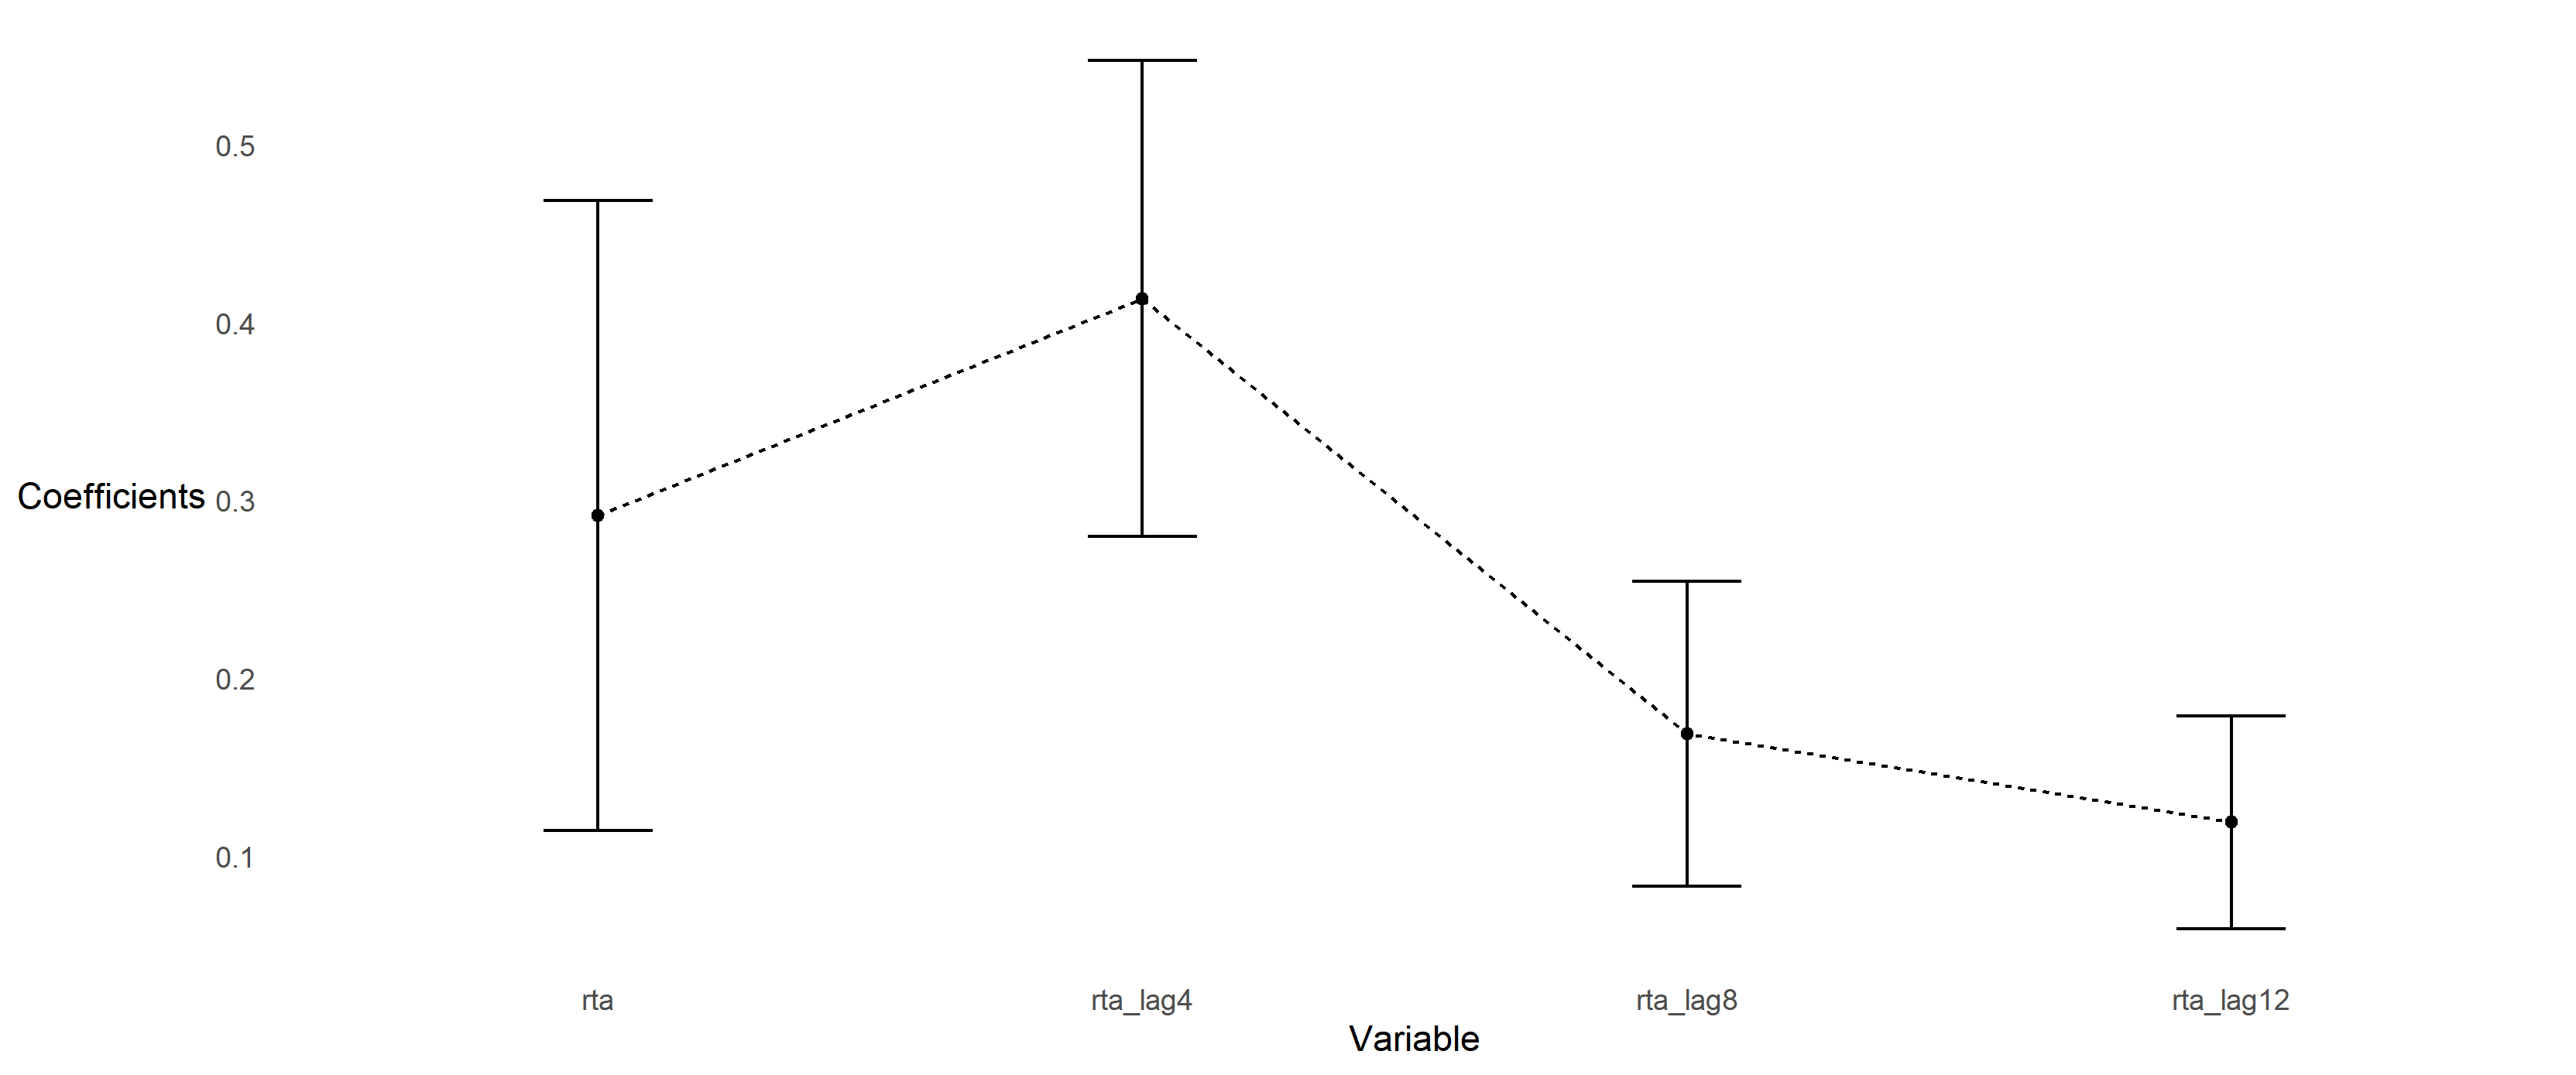
\includegraphics[width=\textwidth]{fig_rta_evo.png}
	\caption{Evolution of RTA impact on trade over time. \newline
		\textbf{Source:} Author's calculations.}
	\label{fig_foreign_born}
\end{figure}


%
%\bibliographystyle{chicago}
%\bibliography{../bibliography.bib}
%
%	
\end{document}